%% This is file `elsarticle-template-1-num.tex',
%%
%% Copyright 2009 Elsevier Ltd
%%
%% This file is part of the 'Elsarticle Bundle'.
%% ---------------------------------------------
%%
%% It may be distributed under the conditions of the LaTeX Project Public
%% License, either version 1.2 of this license or (at your option) any
%% later version.  The latest version of this license is in
%%    http://www.latex-project.org/lppl.txt
%% and version 1.2 or later is part of all distributions of LaTeX
%% version 1999/12/01 or later.
%%
%% Template article for Elsevier's document class `elsarticle'
%% with numbered style bibliographic references
%%
%% $Id: elsarticle-template-1-num.tex 149 2009-10-08 05:01:15Z rishi $
%% $URL: http://lenova.river-valley.com/svn/elsbst/trunk/elsarticle-template-1-num.tex $
%%
\documentclass[final,12pt]{elsarticle}
\usepackage[margin=25mm]{geometry}
\linespread{1.5}

\usepackage{titlesec}
\usepackage{multirow}
\usepackage{siunitx}	% use "s" as column header to line up thousands, decimals etc.
\sisetup{input-ignore={,},input-decimal-markers={.}}
\usepackage{graphics}
\usepackage{booktabs}	% makes tables look a little nicer. Use \toprule \ midrule and \bottomrule
\usepackage{amsmath}
\usepackage{longtable}	% use \begin{longtable} for tables that can span multiple pages



\setcounter{secnumdepth}{4}

\titleformat{\paragraph}
{\normalfont\normalsize}{\theparagraph}{1em}{}
\titlespacing*{\paragraph}
{0pt}{3.25ex plus 1ex minus .2ex}{1.5ex plus .2ex}

%% Use the option review to obtain double line spacing
%% \documentclass[
,review,12pt]{elsarticle}

%% Use the options 1p,twocolumn; 3p; 3p,twocolumn; 5p; or 5p,twocolumn
%% for a journal layout:
%% \documentclass[final,1p,times]{elsarticle}
%% \documentclass[final,1p,times,twocolumn]{elsarticle}
%% \documentclass[final,3p,times]{elsarticle}
%% \documentclass[final,3p,times,twocolumn]{elsarticle}
%% \documentclass[final,5p,times]{elsarticle}
%% \documentclass[final,5p,times,twocolumn]{elsarticle}

%% The graphicx package provides the includegraphics command.
\usepackage{graphicx}
%% The amssymb package provides various useful mathematical symbols
\usepackage{amssymb}
%% The amsthm package provides extended theorem environments
%% \usepackage{amsthm}

%% The lineno packages adds line numbers. Start line numbering with
%% \begin{linenumbers}, end it with \end{linenumbers}. Or switch it on
%% for the whole article with \linenumbers after \end{frontmatter}.

%% natbib.sty is loaded by default. However, natbib options can be
%% provided with \biboptions{...} command. Following options are
%% valid:

%%   round  -  round parentheses are used (default)
%%   square -  square brackets are used   [option]
%%   curly  -  curly braces are used      {option}
%%   angle  -  angle brackets are used    <option>
%%   semicolon  -  multiple citations separated by semi-colon
%%   colon  - same as semicolon, an earlier confusion
%%   comma  -  separated by comma
%%   numbers-  selects numerical citations
%%   super  -  numerical citations as superscripts
%%   sort   -  sorts multiple citations according to order in ref. list
%%   sort&compress   -  like sort, but also compresses numerical citations
%%   compress - compresses without sorting
%%
%% \biboptions{comma,round}

% \biboptions{}

\journal{Journal Name}

\begin{document}

\begin{frontmatter}

%% Title, authors and addresses

\title{Next Generation Urban Search \& Rescue Robot}

%% use the tnoteref command within \title for footnotes;
%% use the tnotetext command for the associated footnote;
%% use the fnref command within \author or \address for footnotes;
%% use the fntext command for the associated footnote;
%% use the corref command within \author for corresponding author footnotes;
%% use the cortext command for the associated footnote;
%% use the ead command for the email address,
%% and the form \ead[url] for the home page:
%%
%% \title{Title\tnoteref{label1}}
%% \tnotetext[label1]{}
%% \author{Name\corref{cor1}\fnref{label2}}
%% \ead{email address}
%% \ead[url]{home page}
%% \fntext[label2]{}
%% \cortext[cor1]{}
%% \address{Address\fnref{label3}}
%% \fntext[label3]{}


%% use optional labels to link authors explicitly to addresses:
%% \author[label1,label2]{<author name>}
%% \address[label1]{<address>}
%% \address[label2]{<address>}

\author{Joseph Flannery $\vert$ Harvey Francis $\vert$ Maximillian Gloger $\vert$ Alex Lamm $\vert$ Daniel Riley $\vert$ Yung-Yu Lau}

\address{University of Warwick}

\begin{abstract}
%% Text of abstract
Bacon ipsum dolor amet turkey meatball frankfurter pastrami filet mignon pork drumstick capicola biltong sausage. Tail pancetta t-bone cupim ground round, filet mignon tongue leberkas. Jerky venison bresaola shoulder boudin ground round sausage turducken biltong bacon salami pancetta brisket hamburger spare ribs. Sausage frankfurter rump kielbasa, pig ham hock tongue picanha sirloin. Chicken turducken short loin andouille, ribeye filet mignon bresaola pork chop beef ribs. Pork loin bresaola turkey pig t-bone.
\end{abstract}
\begin{keyword}
Bacon \sep Pig \sep Sausage
%% keywords here, in the form: keyword \sep keyword

%% MSC codes here, in the form: \MSC code \sep code
%% or \MSC[2008] code \sep code (2000 is the default)

\end{keyword}

\end{frontmatter}

\begin{figure}[h]
\centering\includegraphics[width=\linewidth]{Images/Cyclone.png}
\end{figure}

\pagenumbering{roman}
%\clearpage
%\tableofcontents
%\clearpage
%\listoffigures
%\clearpage
%\listoftables
%\clearpage

%% main text
\pagenumbering{arabic}
%\section{Strategy}
The strategy of the 2015/16 Warwick Mobile Robot team was based around the following points;
\begin{itemize}
\item{Reviewing Orion, the robot from the 2014/15 WMR team and deciding which aspects require redesign and improvement.}
\item{Base our designs for Cyclone on Orion as much as possible so we are able to reuse some of Orion’s components.}
\item{Building bridges between suppliers and others by means of meetings and outreach events to raise awareness of WMR projects and create relationships between relative suppliers for this year's project and for any future WMR projects.}
\item{Completing the project with a fully functioning robotic vehicle which can be used as a basis for next year’s team to make final additions in order enter into competition.}
\end{itemize}
\subsection{Aims and Objectives}
Our aim is to design, test and manufacture an urban search and rescue robot for use in disaster zones to locate and aid trapped survivors, and to raise awareness for the capabilities of search and rescue robots in these situations. \par
To achieve this aim, our objectives this year are as follows;
\begin{enumerate}
\item{To further develop the previous year’s robotic vehicle to improve its functionality and search and rescue capabilities.}
\item{To conclude this project with a vehicle which can be used as a platform for next year’s team to finalise the robot for means of a competition entry.}
\item{To improve the awareness of search and rescue robots and to inspire the next generation to enter into the world of robotics.}
\end{enumerate} \par
\subsection{Team Structure}
This year’s team consisted of six fourth year students from various disciplines within the School of Engineering at the University of Warwick. The engineering discipline distribution was; two mechanical, two mechanical \& manufacturing, an electronic and a systems. \par
The robot chassis was split into three modules and generated  individual tasks for the four mechanical engineering team members; the chassis, drivetrain, suspension and dynamic tension systems. The entirety of the electronics work was performed by the sole electronic engineer in the team and the systems engineer was responsible for communications, both electrical and mechanical. Collaboration between team members was essential throughout this project, especially between the mechanical members due to the large level of overlap between their respective tasks. \par
Each team member also had an administrative role in order to keep the team running effectively and efficiently and to avoid the time of one member of the team being taken up by all of these tasks.. These roles included a project manager, a secretary, a finance director, a sponsorship manager, a social media officer and outreach officer. \par
\subsection{Project Lifetime}
In the time the team had to complete the project, it was clear that there would not be sufficient time to produce a robot that would be able to compete in a competition. The team decided they will build a robot up to a stage where it could be finalised and taken to the competition by the 2016-17 team. It was therefore important that the robotic vehicle produced by the end of this year be well designed and adaptable to avoid rework for next year’s team. \par
There was 30 weeks in total to review Orion, design for Cyclone, manufacture, assemble and produce the technical report for this project. The designs for Cyclone were finalised by week 20 and ready for manufacture by week 24, which was later than planned due to complications. The manufacturing was then completed by week 28 and assembled in the same week ready for testing in week 29. The testing, evaluating and report writing was then completed by the end of week 30. \par
\subsection{Management and Logistics}
The team held regular meetings, with all members initially but it was decided that the attendance of the entire team was not always necessary and was sometimes counterproductive and so most later meetings only involved the team members that were required for the particular discussion topic. There were also weekly meetings with all the team members along with the project supervisor in order to update the supervisor on project progress. This meeting was often attended by a technician in order to provide manufacturing expertise. \par
Google Drive acted as the storage facility for all relevant files, such as manufacturing drawings and CAD files. Meeting minutes were recorded by the secretary and uploaded to the Drive area following the meeting for members to review. In order to ensure that contact was always kept between team members, an instant messaging application called Slack was used to update each other of progress. \par
For the technical report, each section was written using Google Docs so that comments and changes could be easily made to the documents by the reviewers. Once all sections were completed, the full report was compiled using LaTex, and after several iterations, the final report was completed.
\newpage
%\section{Design}
%\subsection{Chassis Evaluation and Redesign}

%%%%%%%%%%%%%%%%%%%%%%%%%%%%%%%%%%%%%%%%%%%%%%%%%%%%%%%
\subsubsection{Chassis Overview}
%%%%%%%%%%%%%%%%%%%%%%%%%%%%%%%%%%%%%%%%%%%%%%%%%%%%%%%
Traditionally, the term Chassis refers to a self-moving subassembly that includes a structure to carry a vehicle’s components, suspension, wheels, the steering system, the brake system and the transmission \cite{Gent09}. The field of robotics, however, often refers to the chassis simply as the structural framework of the robot, a definition adopted by previous WMR teams \cite{WMR15}.\par
The purpose of USAR robots is often to assist in environments too difficult or dangerous for humans to enter. This danger could be from radiation, heat, dangerous chemicals or collapsing structures. It is therefore a necessity that the USAR’s containing structure is designed to be rigid and robust, such that any of the above risks are mitigated as much as possible. A similarly rigid outer shell is often added to ensure that foreign components cannot enter the chassis, such as dirt and liquids that may interfere with the robot’s internal systems. Thus, in the context of USAR, the chassis exists as a container and shield for internal components. Further still, heat dissipation through the chassis allows it to act as a heat sink for energy intensive electronics. \par
Materials choice represents a key factor in the design of a robot chassis. Similar to in the automotive industry, a balance needs to be struck between weight and rigidity. The result is often some combination or choice between steel and aluminium, with other options such as carbon fibre reinforced polymers remaining out of the realms of cost-effectiveness for the foreseeable future \cite{Davies12}. \par
Given the risks of damage in the field, the next important consideration is ease of replacement and fast reassembly. Previous WMR teams have placed importance on the manufacturability of robot’s components, as this will facilitate a finished robot by the end of the project \cite{WMR15}, \cite{WMR14} and makes for simple replacement at the RoboCup competition. Another perspective however, is that a reduction in individual components facilitates more than is possible with simple components \cite{Boothroyd10}, though time to manufacture may increase earlier in the process. \par
Finally, the joining processes must be considered. Even the simplest products may be impossible to manufacture from a single piece \cite{Kalpakjian10}, and though it may be possible with some structures to use a single block of material \cite{mcclean08}, the additional machining costs associated with such a decision often bring this out of the realms of feasibility. Whilst previous WMR teams have justified the use of mechanical fastenings to allow for disassembly and ease of replacement, stress distribution, corrosion and joint degradation could be substantially improved if adhesives can be used where appropriate \cite{Davies12}.

%%%%%%%%%%%%%%%%%%%%%%%%%%%%%%%%%%%%%%%%%%%%%%%%%%%%%%%
\subsubsection{Rationale for Previous Design}
%%%%%%%%%%%%%%%%%%%%%%%%%%%%%%%%%%%%%%%%%%%%%%%%%%%%%%%

A number of goals were outlined in the WMR 2015 report:\par

\begin{longtable}{p{0.2\textwidth} p{0.75\textwidth}}
\textbf{Dimension} &
The overall size of the robot was dictated by building regulations, and an estimation that if the robot sits within a 90\% envelope of door and hallway sizes, it will be capable of turning and manoeuvring through buildings. Minimum internal volume specifications of $3.9 \times 10^{-3} m^3$ were also set, on the premise that there must be enough room for all internal components and extra space for air flow.\\
\textbf{Weight} &
As the robot is to be deployable by one person, 25kg was used as a weight maximum to meet health and safety recommendations on carrying weights. The chassis has been allowed 20\% of this weight, at 5kg. This specification was carried over to the current design.\\
\textbf{Accessibility} &
Access to the battery for fast removal was an important consideration for ease of use as well as health and safety. Li-Ion batteries can be dangerous if used improperly and thus it is important to be able to stop the system in a matter of seconds – 30 in this case.\\
\textbf{Manufacture \& Assembly} &
The team elected to stick to off the shelf components as much as possible to ensure that the robot could be easily assembled and repaired should there be damage to components. For similar reasons, it was dictated that any machining work required should be done from easily sourced materials using simple machining techniques to reduce lead time on replacement components.\\
\textbf{Structure } &
Finally, the team required that the chassis be capable of withstanding a fall force of 650N and a crash force of 250N, based on calculations of acceleration from the two cases and including a large factor of safety.\\
\end{longtable}

%%%%%%%%%%%%%%%%%%%%%%%%%%%%%%%%%%%%%%%%%%%%%%%%%%%%%%%
\subsubsection{Critical Analysis of Previous Design}
%%%%%%%%%%%%%%%%%%%%%%%%%%%%%%%%%%%%%%%%%%%%%%%%%%%%%%%
\paragraph{Dimensions}
The requirements set on dimensions worked well for WMR2015, but the inner workings of the robot were still moderately crammed in. The front and rear of the robot’s chassis were limiting in which components could reasonably fit in and items such as the motor controllers took up a large space in the centre module. It may have been more reasonable to open up the space in the rear of the chassis to make room for the controllers next to the motors themselves.
\paragraph{Weight}
Despite the team’s best efforts, the 2015 chassis weighed in at 5.57kg, 10\% greater than anticipated. This can be put largely down to the 10mm thick, solid baseplate that was used as the basis of the robot’s structure. The testing carried out by the team suggested that MakerBeam\textsuperscript{\textregistered} was more than strong enough to withstand the required forces, and that 10mm thick aluminium represented a far greater strength than needed. A thinner aluminium plate could have been used to achieve the required strengths without the same impact on overall weight. Some weight reduction through machining could have also been achieved to lose the weight in these key areas. This increase in weight inevitably impacts other areas of the robot whilst simultaneously increasing the required torque and slowing the speed of the robot. The shell of the robot was made entirely from 2mm thick aluminium sheets, representing an additional weight gain across the entire chassis.
\paragraph{Accessibility}
The robot’s battery was made easily accessible through a battery attachment that allowed fast clip-in/out. The panel used to do this was easily accessible, but access to the rest of the robot remained slightly more complicated, through a large access panel on the top of the robot. Although the panel itself was large, the arrangement of components meant that for many adjustments, more of the skin would have to be removed anyway.
\paragraph{Manufacture and Assembly}
The use of MakerBeam\textsuperscript{\textregistered} on the robot provided the team with an easy assembly for the robot and enabled the robot to be completed in a short time. However, the desired ease of reassembly was not achieved. This was largely down to the way in which individual, shelf-bought components were assembled together, with small screws and poor joining location choices. Ultimately, whilst parts could easily be sourced for replacement, the changeover itself would take far longer than could be deemed acceptable in a USAR situation, where time is very much of the essence. Furthermore, the MakerBeam\textsuperscript{\textregistered} was, in places, doubled up by the 10mm baseplate, giving no functional benefit and adding to assembly time unnecessarily. It is considered best practice, where assembly is concerned, to removed the need for extra assembly steps if similar materials are used and there is no relative motion between the parts nor need for the parts to be separate \cite{Boothroyd10}. Removing this redundant material would have further brought the weight of the chassis down. \par
Machining work was kept to a minimum, but the machining processes used were less readily available than initially suggested, requiring specialist water jet cutting for a number of mission-critical components. The materials used were, fortunately, readily available, limiting sourcing issues. \par
Ultimately these considerations are a product of the team’s goals. Entering a competition for search and rescue robots is a good opportunity to benchmark the performance of the robot, but if decisions are made based on performance in a competition and not performance in a search and rescue environment, then arguably the team have missed the entire point of the project.\par
\paragraph{Structure}
The rationale and justification for the structure chosen was achieved through physical testing of materials and simulation of crash situations. The only physical testing carried out, however, was a 3-point bending test on steel, aluminium and maker beam. This test, whilst useful for some situations, does not accurately represent the load conditions likely to be experienced by the chassis from drops or crashes, where the forces experienced are far more complex than those represented. It is, therefore, far more prudent to carry out simulations of chassis design in Solidworks\textsuperscript{\textregistered}, as is later done. The 3-point bending test should not have been used as the rationale for material choice, especially when MakerBeam\textsuperscript{\textregistered} performed significantly worse than the other materials used (different volumes of materials were also used for the materials resulting in a skewed test, even though the resulting factors were discussed qualitatively).

%%%%%%%%%%%%%%% End of Finished Work %%%%%%%%%%%%%%%%%%


\subsection{Banter}

%\subsection{Drivetrain}
\subsubsection{Rescue Robot Drivetrain}
The drivetrain is the system in a motor vehicle which connects the transmission to the drive axle. In regard to a rescue robot the drivetrain is made up of the motors (and their controllers), the drive axles, the cams (drive wheels), the tracks and all parts in-between. The drivetrain of the rescue robot is a crucial component as without it the robot would have no mobility.\par
The balance between power and speed must also be well thought out. Too little power would mean the robot would be unable to traverse the uneven surfaces of disaster zones and not enough speed would result in a prolonged time to survey and manoeuvre within a disaster zone. The drivetrain of rescue robots are usually tracked rather than wheeled in order to navigate unpredictable terrain. This makes rescue robot control unique.

%Rational of Previous Design%
\subsubsection{Rational of Previous Design (2014/15)}
The drivetrain of Orion (2014/15) was modelled by breaking the design down into three sections; steering, suspension and tracks. These three separate sections ultimately dictated the requirements for their drivetrain and will therefore be used as a basis to review the design of last year’s drivetrain.\par

The steering was designed with the intention of using a skid method which uses two separate motors (one per track) allowing each track to be controlled independently, this is known as dual drive. The skid steering method is one of the more efficient ways of controlling a tracked vehicle as it allows continuous movement whilst turning. The selection behind the steering was sound and the dual drive, skid steering will be used in Cyclone’s (2015/16) design.\par

The tracks were chosen using consultation from experts at Transdev (the track supplier) and analysis of previous designs of WMR robots. Specialist rubber tracks were selected for Orion due to the high durability and traction, and multi-terrain capability. The track layout was also designed with the intention of making Orion invertible (able to drive when flipped over).\par

The motors for Orion were selected using values of worst case acceleration and power required. These conditions were accelerating at 0.3$ms^-2$ up an incline of 38\textordmasculine (the incline of a standard step) with an estimated robot weight of 25kg. These values gave a required torque of 4.95Nm per motor. This resulted in the EC-4pole 22 \o22 mm, brushless, 90 Watt (specification found in Appendix) motor being selected. A gearhead was required to work alongside this motor to reach the torque required. This gearhead was selected to meet the torque requirements of the Orion project (4.95Nm) and can be seen in the Appendix. The location of Orion’s motors were selected with the premise of saving space, allowing more room to locate other components, in particular the sensor array, they were therefore positioned towards the back of the robot (figure \ref{fig:Orionmotorlayout}).\par

%Insert figure XX1 'Orion (2015/16) internal motor layout' (center aligned)%
\begin{figure}[h]
\centering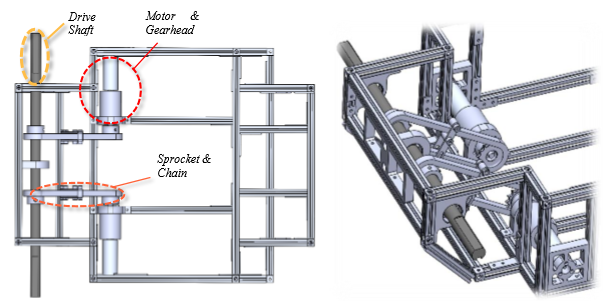
\includegraphics[width=0.6\linewidth]{Images/DT_Fig_1.png}
\caption{Orion (2015/16) internal motor layout}
\label{fig:Orionmotorlayout}
\end{figure}

The RPM required of the motor was governed by the competition specifications which were to accelerate at 0.3$ms^-2$ and have standard operation at 1$ms^-1$. Using the speed constant of Orion’s motors ($907 rpmV^-1$) and the battery’s maximum (24V) and minimum (18V) voltage the speed operating window can be obtained, this is 81.76-109.02rpm and 0.43-0.57$ms^-1$. This was below the  standard operating condition.\par

\subsubsection{Critical Analysis of Previous Design (2014/15)}
The design and reasoning behind the steering system was sound and was the only real option for the type of dual tracked robot that is being built in this project. Using separate motors to control each track will give enhanced mobility and will allow for a more fluid movement than if one motor was used. This design is also the simplest method of control as it does not involve a clutch or gearing system like the alternatives. Thus, the dual drive method of controlling the robot will be carried forward into Cyclone (2015/16).\par

The material selection for the tracks was sensible and the use of the expertise of the Transdev team will be used to select the tracks for Cyclone (2015/16). The specialist rubber design gives the tracks the flexibility they need not only to travel around the drive wheels and guide wheels but also to react to the uneven terrain of a disaster zone. This in conjunction with our new suspension design will allow for improved traction when traversing this uneven terrain. The track design of Orion was also created with the intention of allowing it to drive when upside down, this meant that it encompasses the area around the body. This invertible design would be void if their suggestion of improvement by the addition of a robot arm was carried out, this would obviously not allow the robot to travel both the right way up and upside down. After consideration of the profile of Orion’s track design it was made clear that the tractive length was too short to allow the robot to climb stairs. The distance between the two points of consecutive steps is 308.8mm (figure \ref{fig:Orionstairs} and \ref{fig:Cyclonestairs}) and the tractive length of Orion was only 244.60mm, whereas Cyclone’s new extended parallelogram track profile allows it to easily climb a standard step (figure \ref{fig:Cyclonestairs}).\par

%These figure are on the same level%
%Insert figure XX2 'Orion struggling to climb standard stairs',(left aligned)%
%Insert figure XX3'Cyclone easily climbing standard stairs', (right aligned)%
\begin{figure}[h]
\centering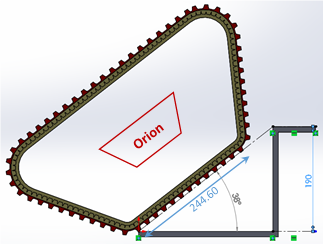
\includegraphics[width=0.5\linewidth]{Images/DT_Fig_2.png}
\caption{Orion struggling to climb standard stairs}
\label{fig:Orionstairs}
\end{figure}

\begin{figure}[h]
\centering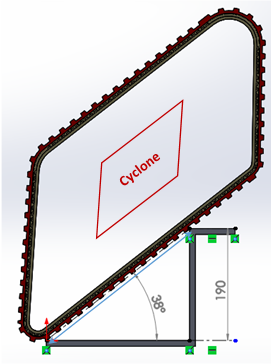
\includegraphics[width=0.4\linewidth]{Images/DT_Fig_3.png}
\caption{Cyclone easily climbing standard stairs}
\label{fig:Cyclonestairs}
\end{figure}

As mentioned in the previous section the motor and gearhead combination were selected using the worst case scenario of accelerating a 25kg Orion at 0.3$ms^-2$ up an incline of 38\textordmasculine. This calculation gave a required torque of 4.95Nm per motor. This torque was found by assuming 80\% efficiency of the motor and gearhead combination, when in fact the selected motor was 88\% efficient and the gearhead was 77\% efficient giving a total efficiency of 67.76\%. Using the actual efficiency, the worst case scenario torque required for Orion would be 5.79Nm. This highlights the point that the efficiency should have been thoroughly researched and a sensible estimate made from the Maxon Motor data available. The stall torque was also taken into consideration and so a motor with a minimum stall torque of 25Nm was suggested (about five timed times the worst case torque). With this in mind a motor with a stall torque of 0.588Nm and a gearhead with a 123:1 reduction were selected giving an overall torque output of 72.32Nm (if 100\% efficiency and maximum running is assumed). Orion has a system with 67.76\% efficiency and so therefore, using the nominal current and torque constant for Orion’s motors, one can see that this combination is not suited for accelerating the 25kg Orion up a 38\textordmasculine slope as it only provides 3.45Nm rather than the 5.79Nm required. Further analysis using a simple force diagram (figure \ref{fig:slopeforce}) shows that a total force of 150.99N is required to hold a weight of 25kg still on a 38\textordmasculine slope. This equates to 75.5kg and 3.77Nm per motor, which is greater than the torque that Orion’s motors provide. The motor and gearhead selected for Orion will render the robot useless whenever it comes to any obstacle.\par

%Insert figure XX4 'Simple force diagram for Orion on a 38deg slope' (center aligned)%
\begin{figure}[h]
\centering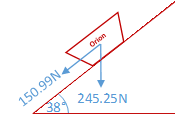
\includegraphics[width=0.4\linewidth]{Images/DT_Fig_4.png}
\caption{Simple force diagram for Orion on a 38\textordmasculine slope}
\label{fig:slopeforce}
\end{figure}

The speed of the motors was also lacking, only giving a maximum speed of 0.57$ms^-1$. This speed would not be maintained as this was calculated assuming the battery had maximum charge. Realistically the speed would be more around the lower value of 0.43$ms^-1$.\par

There is always a trade-off between speed and torque but it is hard to see here which factor was favoufavouredred  in the design of Orion’s drivetrain, as neither the speed nor the torque are sufficient for the successful operation of the robot. For this reason a new motor and gearhead selection will be made for Cyclone.\par

%Review of Alternative Drivetrain Designs%
\subsubsection{Review of alternative Drivetrain Design}

There are a number of different methods that can be used to propel a vehicle, this section will explore a number of options and justify the option chosen.\par

\paragraph*{Propulsion}

Firstly, the robot needs a way of converting power to forward momentum. Choosing the best system depends on several factors including the traction, steering, suspension and the ground pressure. Three methods of delivering movement were explored; wheels, tracks and legs.\par

\subparagraph*{Wheels}
%insert reference for this section http://www.intorobotics.com/wheels-vs-continuous-tracks-advantages-disadvantages/%
This is the most common method of movement in ground vehicles and so the possibility was explored for Cyclone.\par

Wheels provide a simple platform for movement as there are limited moving parts involved, namely only the wheel and drive axle will be turning. This means that there are fewer components that could get damaged. If there was ever any damage however, the simplicity of design would mean the repair would be quick, easy and cheap. This simplicity would also mean constructing a wheeled robot, including the suspension element, would be easier and cheaper than a more complicated design such as a tracked variant.\par

The wheeled design offers a high degree of manoeuvrability and allows the robot to travel at high speeds compared with tracks and legs, this due to the wheels needing a lower torque to start and continue moving. This high degree of manoeuvrability also makes the wheeled robot easy to control. Figure \ref{fig:wheelturn} shows the method of turning for a wheeled vehicle, the robot can turn on the spot by driving the left wheels forward and the right wheels backwards. The steering of a wheeled robot could also be carried out using the same method as a car (bell-crank and rack-and-pinion steering linkage).\par

%Insert figure XX5 'Turning Method of a wheeled robot' (center aligned)%
\begin{figure}[h]
\centering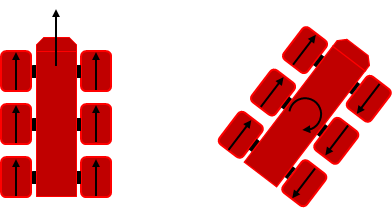
\includegraphics[width=0.6\linewidth]{Images/DT_Fig_5.png}
\caption{Turning Method of a wheeled robot}
\label{fig:wheelturn}
\end{figure}

Because wheels have been around for such a long time they have seen a number of advancements in their design and so there are a number of variants of the wheel, shown below (Figure \ref{fig:Wheeltype}).\par

%Insert figure XX6 'Different Wheel types for a Robot' (center aligned)%
\begin{figure}[h]
\centering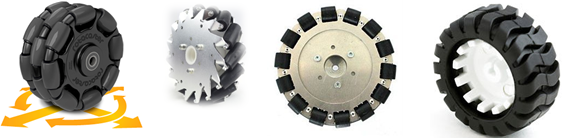
\includegraphics[width=0.6\linewidth]{Images/DT_Fig_6.png}
\caption{Different Wheel types for a Robot}
\label{fig:Wheeltype}
\end{figure}
%References for figure (left to right: Omni https://en.wikipedia.org/wiki/Omni_wheel%
%mecanum http://robu.in/shop/152mm-aluminium-mecanum-wheel-right/%
%omnidirectional http://www.robotshop.com/en/152mm-omnidirectional-wheel.html%
%standard https://www.sparkfun.com/products/8899%

Although they have a large variety of designs available and their simplicity makes them cheap and easy to build wheels do have their disadvantages. The first and main disadvantage is that wheels must be at least twice the height of an obstacle in order to overcome it, so in the case of climbing a standard staircase the wheel must be 380mm high. The second major disadvantage is the small contact area with the ground resulting in reduced traction. This small contact area also means the weight is concentrated at specific points making wheeled vehicles unsuitable for soft terrain.\par

\subparagraph*{Tracks}
%insert reference for this section http://www.intorobotics.com/wheels-vs-continuous-tracks-advantages-disadvantages/%

Tracks are an alternative to the wheeled design although they offer a more complex system. Unlike a wheeled design tracks have a low ground impact as the weight is distributed along the track length in contact with the ground. This is ideal for a disaster zone where survivors may be trapped under rubble. The larger footprint of the track offers increased traction and therefore a higher performance efficiency compared to wheels. The increased traction coupled with the flexibility of the continuous tracks also allows for the traversing of rough terrain where a wheeled design would get stuck due to its single contact points.\par

The steering system is as simple as the wheeled design (figure \ref{fig:trackturn}) allowing for on the spot turning and good manoeuvrability.\par

%Insert figure XX7 'Turning Method of a tracked robot' (center aligned)%
\begin{figure}[h]
\centering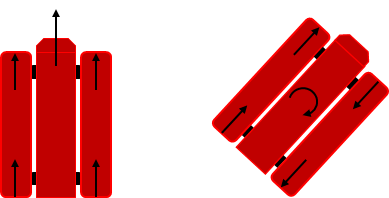
\includegraphics[width=0.6\linewidth]{Images/DT_Fig_7.png}
\caption{Turning Method of a tracked robot}
\label{fig:trackturn}
\end{figure}

Although the tracked design is better suited to the rough terrain of a disaster zone it does offer less precise movement and due to the increased traction more power is required whilst turning. The overall design tends to be bulky and heavier and given the more complex nature the build and repair tend to be more costly than alternatives.\par

\subparagraph*{Legs}
%insert reference for this section https://www.quora.com/Is-there-any-benefit-to-legged-robots-over-wheeled-ones%

Legs are becoming more and more common in robot designs and so they were considered for Cyclone.\par

Legs are the most agile of the three options and rather than being able to perform at high speeds they enable the robot to react quickly to any outside forces or changes in environment, allowing a change in pose or principal orientation. This reactiveness allows for an extremely stable platform for the robot when walking over ice, mud, rocks etc. A legged robot also has the advantage of the environment being designed specifically for legged/limbed locomotion (humans). Limbs (of a robot) also allow a greater ‘solution space’ giving more options when traversing uneven surfaces and obstacles (figure \ref{fig:solutionspace}). The limbs of the robot could also be utilised to climb vertical surfaces allowing the exploration of areas tracked or wheeled robots could not reach (figure \ref{fig:legclimb}).\par

%Insert figure XX8 'Solution Space of a legged robot' (center aligned)%
\begin{figure}[h]
\centering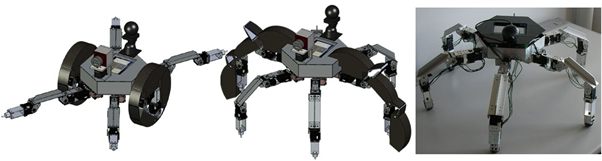
\includegraphics[width=0.6\linewidth]{Images/DT_Fig_8.png}
\caption{Solution Space of a legged robot}
\label{fig:solutionspace}
\end{figure}
%Insert figure XX9 'Legged Robot Climbing a vertical surface' (center aligned)%
\begin{figure}[h]
\centering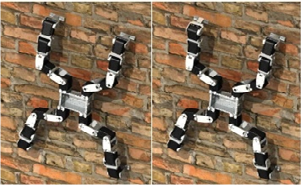
\includegraphics[width=0.6\linewidth]{Images/DT_Fig_9.png}
\caption{Legged Robot Climbing a vertical surface}
\label{fig:legclimb}
\end{figure}

As well as the physical advantages, a limbed robot would be a more sensible choice in terms of set-up and cost for a disaster extraction, because no local infrastructure would have to be set up, like paths and open passages.\par

The limb design is still in research and so is currently expensive and extremely time consuming to get right on a project dealing with such unpredictable environments. This is the main downfall of this type of design.\par

\subparagraph*{Choice}

Considering the three options above the best choice for Cyclone would be a tracked drivetrain. The main reason for this is because of its more rugged nature and greater ability to traverse the uneven terrain it will encounter in a disaster zone.\par

\paragraph*{Manoeuvrability}

The method of steering is the next factor to consider now that tracks have been selected for the drivetrain. There are a number of way to steer a two track vehicle and this section will explore five options and ultimately decide the best of these.\par
%Not all of these need to be in the text, a couple can go in the appendix%

\subparagraph*{Dual Drive}

This is the simplest way to steer a dual tracked vehicle and requires a separate power source (motor) for each track.\par

In order to steer this system one motor is supplied with more power than the other, this results in one track travelling faster (and so further) than the other causing a turning moment. This design also allows the vehicle to perform a neutral turn (turn on the spot) by driving one motor forward and the other in reverse. This will be useful when navigating the tight environment of a disaster zone. The simplicity of the design make the steering intuitive and so the vehicle is easy to operate often using one throttle ‘stick’ per motor, allowing any unskilled personnel to pick up a controller and operate the vehicle.\par

This design does come with some disadvantages. Two power sources means double the chance of something going wrong and so reliability will be lower than a system with one motor. If one motor was to fail the vehicle would be immobilised and capable of only spinning in circles, rendering it useless. Another issue with two motors is there will be double the weight, and with the motors tending to be near the drive wheels (at the back) this presents an issue with the centre of gravity. The final issue would be the ease of steering. It may be difficult to supply the same amount of power through each motor and still maintain a straight line. If the same power is supplied to each motor to travel in a straight line, there would still be the issue of each track not experience the same amount of drag causing the tracks to turn at slightly different speeds. This tends not to be an issue at lower speeds.\par

%Insert figure X10 'Dual Drive Layout' (center aligned)%
\begin{figure}[h]
\centering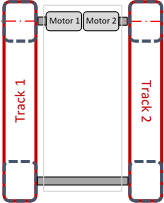
\includegraphics[width=0.4\linewidth]{Images/DT_Fig_10.png}
\caption{Dual Drive Layout}
\label{fig:dualdrive}
\end{figure}

\subparagraph*{Clutch Brake}

This method only requires one motor which drives both tracks directly. This technique involves disengaging one track from the motor via a clutch mechanism (figure \ref{fig:clutchbrake}) in order to slow the disengaged track until it comes to a stop. The other track is still engaged and traveling at the speed of the motor, so causing a turning effect. The disengaged track can also use a brake to bring it to an immediate stop allowing a tighter turning radius. This is another easy method of controlling a tracked vehicle it is however not very efficient. The constant stopping and accelerating of the tracks also makes manoeuvring slow and inefficient, because by slowing and braking one track in order to turn energy is wasted from the motor. This method also does not allow on the spot turning which would cause problems in the tight areas within a disaster zone.\par

%Insert figure X11 'Clutch Brake Layout' (center aligned)%
\begin{figure}[h]
\centering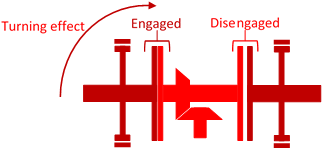
\includegraphics[width=0.6\linewidth]{Images/DT_Fig_11.png}
\caption{Clutch Brake Layout}
\label{fig:clutchbrake}
\end{figure}

\subparagraph*{Gearing Steering}

In a gearing steering system a single motor is used to power both sets of tracks through separate transmissions. The tracked vehicle is steered by selecting different gears for each of the tracks. In figure \ref{fig:gearSteer} the $1^{st}$ gear is engaged on the left side and the $2^{nd}$ gear is engaged on the right side, this will result in the left track travelling at a lower speed than the right and so giving a left hand turning effect. This method allows for a smooth and efficient method of steering the vehicle and allows a large combination of gearing ratios to be used for a large number of turning radii. Another advantage of this method is that each transmission can incorporate a reverse gear and so a neutral turn is possible. However, this method is complex in nature and correct implementation can be time consuming and costly.\par

%Insert figure X12 'Gearing Steering Layout' (center aligned)%
\begin{figure}[h]
\centering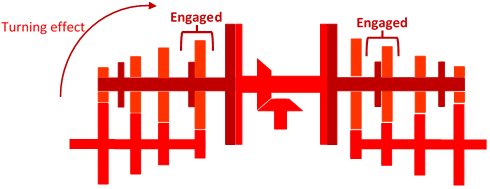
\includegraphics[width=0.6\linewidth]{Images/DT_Fig_12.png}
\caption{Gearing Steering Layout}
\label{fig:gearSteer}
\end{figure}

\subparagraph*{Braked Differential}

This is a simplified version of the clutch-brake drive shown above. The two axles are driven through a differential and so eliminating the clutches. When one axle is slowed or stopped the differential acts to transfer all the motion to the remaining ‘free’ axel and so resulting in a turning effect. This method is however less efficient than the clutch-brake system, given the brake dissipates the energy of the track and the motor. The braked differential method is also harder to control and straight line travel may become a problem as the system can become unpredictable. However, Its simplicity makes up for these faults.\par

%Insert figure X13 'Braked Differential Layout' (center aligned)%
\begin{figure}[h]
\centering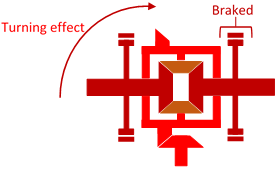
\includegraphics[width=0.6\linewidth]{Images/DT_Fig_13.png}
\caption{Braked Differential Layout}
\label{fig:brakeddiff}
\end{figure}

\subparagraph*{Double Differential}

This is a more refined version of the standard braked differential system. This method adds a second transmission between the steering input of the transmission and the motor. This allows the differential gears to be run at several different speeds resulting in a large combination of track speeds. This will allow for a great number of turning radii making this system extremely well suited for fast steering vehicles. This system is used for all modern fast track-layer steering transmissions due to its efficiency, turning radii possibilities (including a neutral turn) and its stability (it won’t self-steer).\par

%Insert figure X14 'Double Differential Layout' (center aligned)%
\begin{figure}[h]
\centering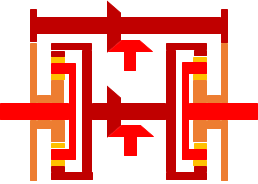
\includegraphics[width=0.4\linewidth]{Images/DT_Fig_14.png}
\caption{Double Differential Layout}
\label{fig:doublediff}
\end{figure}

\subparagraph*{Choice}

Due to the simplicity of its design and the ease of use the dual drive option was chosen to power Cyclone.\par

\subsubsection{Design of Cyclone's Drivetrain}

Cyclone’s drivetrain was created from scratch given the new modular design implemented for this build and the drawbacks of the previous year’s design. Within the modular build the rear module is solely dedicated to the drivetrain. As mentioned above tracks were chosen along with a dual drive system for Cyclone allowing it to easily traverse the unpredictable terrain found within a disaster zone.\par

The motors for Cyclone were considered against the amended worst case requirements, this is accelerating 30kg at 0.3$ms^-2$ up an incline of 38\textordmasculine. Cyclone is predicted to have a slightly heavier weight of 30kg as its design is intended to be added to in future projects and so taking into account a heavier weight will allow the same drive system to be used in the future.\par

According to the simple force diagram (figure \ref{fig:simpleforcecyclone}) Cyclone will require a force of 181.19N to keep it stationary on an incline of 38\textordmasculine, that is 90.59N per motor.\par

%Insert figure X15 'Simple force diagram for Cyclone on a 38deg incline' (cneter aligned)%
\begin{figure}[h]
\centering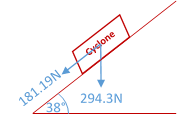
\includegraphics[width=0.4\linewidth]{Images/DT_Fig_15.png}
\caption{Simple force diagram for Cyclone on a 38\textordmasculine incline}
\label{fig:simpleforcecyclone}
\end{figure}

The minimum amount of torque required in this worst case scenario can be found by simplifying figure \ref{fig:simpleforcecyclone} to a wheel travelling up a slope (figure \ref{fig:simpleforcewheel}).

%Insert figure X16 'Simple force diagram for a wheel on a 38deg incline' (cneter aligned)%
\begin{figure}[h]
\centering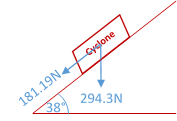
\includegraphics[width=0.4\linewidth]{Images/DT_Fig_16.png}
\caption{Simple force diagram for a wheel on a 38\textordmasculine incline}
\label{fig:simpleforcewheel}
\end{figure}

A force balance using figure \ref{fig:simpleforcewheel} will give the following equation,
\begin{equation}
\sum F_x=F-mgsin\Theta = ma
\end{equation}

Torque ($\tau=F \times r$) can then be substituted into equation D1 and rearranged to get an equation for the torque up an incline.
\begin{equation}
\tau=(a+gsin\Theta)mr
\end{equation}

Given that there are two motors powering Cyclone working at an efficiency below 100\% this should be accounted for and so equation D2 should be divided by the number of motors ($n$) multiplied by their efficiency ($\epsilon$),
\begin{equation}
\tau= \frac{(a+gsin\Theta)mr}{n \epsilon}
\end{equation}

In order to complete this equation the efficiency of the motors and gearhead combination must be estimated. This was done by using the Maxon Motor website and the average efficiencies of likely motors and gearheads that Cyclone would use. The efficiency was estimated to be 60\%, this gives the following result for torque required,
\begin{equation}
\tau= \frac{(0.3+9.81sin38) \times 30 \times 0.05}{2 \times 0.6} = 7.79 Nm
\end{equation}

That is 7.79Nm per motor to accelerate 30kg at 0.3$ms^-2$ up an incline of 38\textordmasculine. The same formula could be used with $a=0 ms^-2$ for Cyclone being held still on the slope, this gives a torque of 7.55Nm (the stall torque).\par

The speed requirement for Cyclone is modified from the previous 2014/15 Orion project, which required a standard operation speed of 1$ms^-1$. This seemed ambitious given the motor and gearhead combinations available and their torque requirement. This prompted the speed requirement to be lowered to $0.5ms^-1$ standard operation, which is more achievable. From this information five motor and gearhead combinations were selected outlined in table \ref{tab:MotorGearSpec}.\par

\begin{table}[h]
\centering
\resizebox{\linewidth}{!}{
\begin{tabular}{p{4cm} s s s s s s s s s}
\hline
Type & Option & \multicolumn{2}{s}{Nominal Speed} & Nominal & Stall & Max Combined  & Gear  & Cost per.  & Length \\
\cline{3-4}
 & & Min V & Max V & Torque & Torque & Efficiency (\%) & Reduction & Combination & \\
\hline
EC 45dia. 15W w/ hall sense w/ GP42C 126:1 gearhead & 1 & 0.21 & 0.25 & 13,1412 & 1540 & 57.6 & 126 & £554.15 & 215.6\\
EC 45dia. 15W w/ hall sense w/ GP42C 126:1 gearhead & 2 &  0.19 & 0.26 & 13,279 & 1600 & 57.6 & 126 & £554.15 & 215.6 \\
RE50 200W 24V GB motor w/ GP52C 26:1 gear & 3 & 0.29 & 0.38 & 8,677.44 & 7370 & 78.02 & 26 & £460.21 & 206.4 \\
EC-4 pole 30dia. 200W 48V w/ GP42C 126:1 gearhead & 4 & 0.17 & 0.22 & 8,292.82 & 3430 & 64.8 & 126 & £505.63 & 155.2 \\
EC-4 pole 30dia. 200W 48V w/ GP32HP 123:1 gearhead & 5 & 0.17 & 0.22 & 7,870.5 & 3430 & 63 & 123 & £526.09 & 155.2 \\
\hline
\multicolumn{10}{c}{Orion's (2014/15) selection} \\
\hline
EC-4 pole 22dia. 200W 48V w/ GP32C 123:1 Gearhead & - & 0.43 & 0.57 & 3,436.84 & 588 & 61.6 & 123 & £718.70 & 122.7 \\
\hline
\end{tabular}
}
\caption{Motor and Gear head specification and selection}
\label{tab:MotorGearSpec}
\end{table}
%$^1$ The options were ranked by 1nominal Torque in descending order.}
%$^2$ The Nominal speed was found by the following equation, ((V×(speed constant)×efficiency)/(gear reduction)). Max V is the maximum voltage that the motor could run at and Min V is the minimum voltage (varies with motors).
%$^3$ The Nominal torque was found using the following equation, (nominal current×torque constant×gear reduction×efficiency).
%$^4$ Stall torque is obtained from the motor specification from Maxon Motor. [RefMotor]
%$^5$ Maximum combined efficiency is found by, (motor efficiency ×gear head efficiency).
%$^6$ Gear Reduction is obtained from the motor specification from Maxon Motor. [RefMotor]
%$^7$ Cost per combination is obtained from the motor specification from Maxon Motor adding cost of motor to cost of gear head. [RefMotor]
%$^8$ Length is obtained from the motor specification from Maxon Motor adding length of motor to length of gear head. [RefMotor]
%RefMotor - http://www.maxonmotor.co.uk/maxon/view/content/index%

As can be seen from table \ref{tab:MotorGearSpec}, the most appropriate motor given the design specifications for Cyclone is the 3rd choice, RE50 200W 24V GB motor with GP52C 26:1 gearhead. This motor does not have as high a torque as option 1 or 2 but does have the highest speed, the greatest stall torque, the best efficiency and is the cheapest option. This option however does not meet the speed requirement of 0.5$ms^-1$. This compromise was accepted on the grounds that the robot must be able to traverse the uneven terrain of a disaster zone and so torque should take priority. As seen in table \ref{tab:MotorGearSpec} the nominal torque (maximum continuous torque) of the chosen combination is 887.44Nm above that of the worst case torque required.\par

%These figure are on the same level%
%Insert figure X17 'Maxon Motor Gearhead, Part no. 370356' (Left aligned)%
\begin{figure}[h]
\centering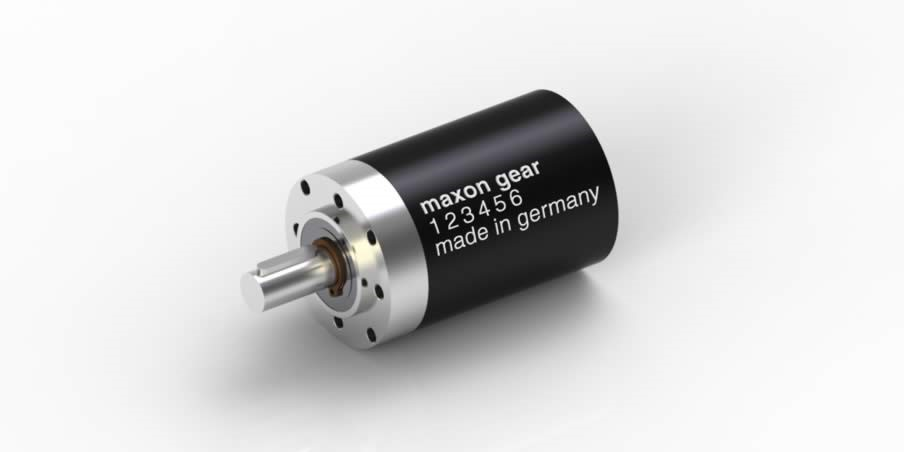
\includegraphics[width=0.6\linewidth]{Images/DT_Fig_17.jpg}
\caption{Maxon Motor Gearhead, Part no. 370356}
\label{fig:gear}
\end{figure}
%Insert figure X18 'Maxon Motor, motor, Part no. 223087' (Right aligned)%
\begin{figure}[h]
\centering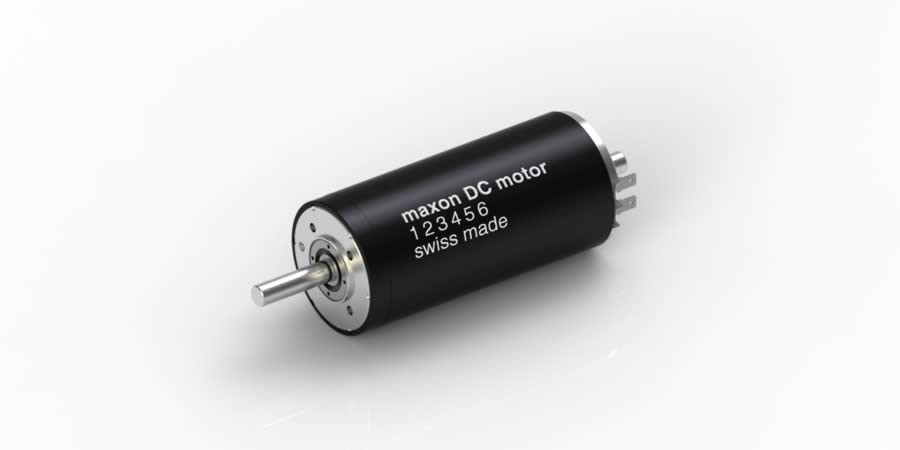
\includegraphics[width=0.6\linewidth]{Images/DT_Fig_18.jpg}
\caption{Maxon Motor, motor, Part no. 223087}
\label{fig:motor}
\end{figure}

The efficiency of this motor and gearhead combination is 78.02\% and therefore the calculation for the torque required to accelerate 30kg at 0.3$ms^-2$ up an incline of 38\textordmasculine can be revised using this new efficiency (equation D5).\par
\begin{equation}
\tau= \frac{(0.3+9.81sin38) \times 30 \times 0.05}{2 \times 0.7802} =6.09 Nm
\end{equation}

That is 6.09Nm per motor for this worst case scenario. The same formula again could be used with $a=0ms^-2$ for Cyclone being held still on the slope, this gives a torque of 5.81Nm (the stall torque). This shows that the motors more than meet the torque requirements of Cyclone.\par

%References- 
%[Ref1] - http://www.intorobotics.com/wheels-vs-continuous-tracks-advantages-disadvantages/
%[Ref2] - https://www.quora.com/Is-there-any-benefit-to-legged-robots-over-wheeled-ones
%[Ref3] - http://www.astro.mech.tohoku.ac.jp/~eric/sitePages/leon.html
%[Refrandom] - http://www.simbotics.org/files/pdf/drivetraindesign.pdf
%[Refrandom] - https://en.wikipedia.org/wiki/Steering
%[RefSkidsteer] - http://groups.csail.mit.edu/drl/courses/cs54-2001s/skidsteer.html
%[RefAlternativeDrivetrain] - http://www.altfuels.org/backgrnd/altdrive.shtml
%[RefSteering] - http://www.gizmology.net/tracked.htm
%[RefMotor] - http://www.maxonmotor.co.uk/maxon/view/content/index

%\subsection{Suspension}
\subsubsection{Why Use Suspension?}
Suspension allows relative motion between the body of a vehicles and its wheels. This motion improves road holding by allowing the wheel and tyre to track the contours of the ground keeping the tyre in contact. Suspension also isolates the body of the vehicles from the uneven road surface, improving ride quality and comfort. Vibration and impacts on the vehicle are also reduced lowering the stress on components thus improving lifespan and reliability \cite{Jazar09}. Overall, the use of suspension allows a vehicle to travel faster and more safely over rough terrain. Less energy is lost from the vehicle moving vertically and less energy is lost from the wheels spinning in mid-air.

\subsubsection{Rationale of Previous Design}
The suspension design of the 2014-2015 version of Orion was a single-pivot swing arm design. A swing-arm rotates around a pivot at one end, whilst suspension is provided by a coil spring mounted part way along the swing arm. As the swing-arm rotates around the pivot the coil spring compresses, absorbing impacts. The idler assembly was mounted to the end of the swing-arm and also allowed to pivot to better conform to terrain. The coil spring was a “coil over damper” type with adjustable preload. The design was chosen because it had been proven in a larger scale in the Ripsaw EV1 \cite{Howe09}. The coil spring suspension design gave a travel of 12mm (approximately half of the maximum spring compression of 25mm), the design has ground clearance of 100mm.

\subsubsection{Critical Analysis of Previous Design}
The most glaring issue with the previous suspension design is that it function is compromised due to a number of factors. The coil spring design was said to have 12mm of travel, however the actual suspension travel is 0mm. This is because sag was seemingly missed from suspension calculations. Sag is compression of the suspension when the vehicle sits on the ground. The robot’s suspension sags and allows a bolt head to contact the outer plate of the suspension mount, stopping the suspension from compressing at all (this can be seen in Figure \ref{fig:LHOrion}). \par
Suspension preload can be increased so that sag is mostly eliminated however, travel is still severely limited due to the bolt fouling against outer mounting plate. \par
\begin{figure}[h]
\centering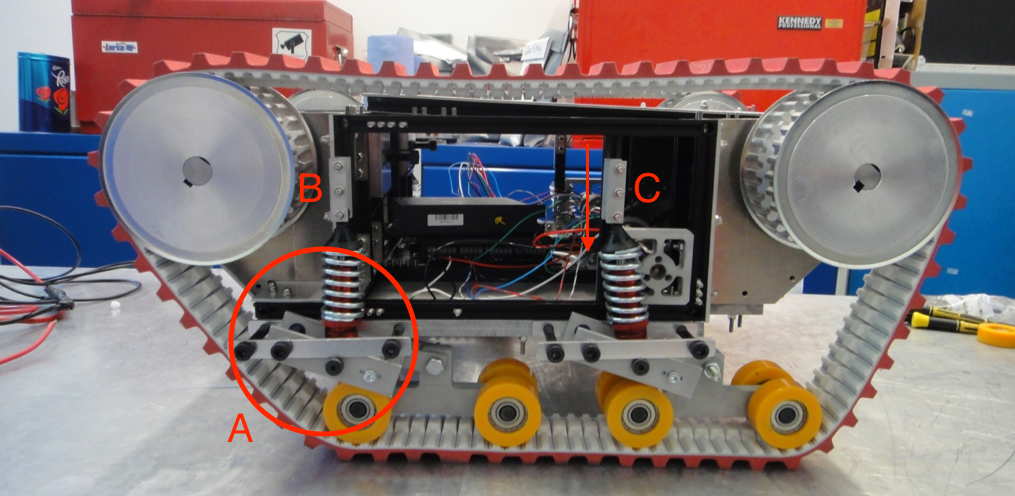
\includegraphics[width=0.6\linewidth]{Images/MaxImages/LHOrion.png}
\caption{Left Hand Suspension from 2014/2015 Technical Report}
\label{fig:LHOrion}
\end{figure}
The design and mounting of the outer mounting plates also cause problems. As can be seen in Figure \ref{fig:LHOrion}  there is no spacer between the inner and outer mounting plates. When the mounting bolts (A on the image) are tightened they bend the outer mounting plates inwards towards the robot. This bending increases frictions as the swing-arm pivot and traps the swing-arm preventing it from rotating.\par

The mounting blocks for the top of the coil spring are also flawed. The are bolts holding them to the MakerBeam chassis elements are perpendicular to the force of suspension compression, there is not restraint in the axis of compression. This means that under high compression events, e.g. a drop from 350mm, the mounting block slips upwards, further any suspension travel to zero. It was found that moving the mounting blocks downwards, illustrated as C in Figure \ref{fig:LHOrion}  rotated the swing-arm so that the spring mounting bolt would not foul the outer mounting plate under compression. This set-up is not ideal however, as it raises the ride height and centre-of-gravity significantly.\par

The suspension assemblies are mounted to the baseplate of the robot with three M6 bolts. When the robot is dropped from the test height of 350mm all of the impact force will be transferred into the baseplate via the four sets of three bolts as none of the energy will be absorbed by the suspension as it cannot compress due to design limitations. The thread depth is 20mm and the length of unsupported bolt is 41mm. Repeated loading of these bolts is likely to damage the shallow threads in the aluminium baseplate, rendering it unusable. \par

Due to the design of the suspension the outer mounting plates and bolts sit outside the outer line of the tracks, shown in Figure \ref{fig:OrionFront}. This makes the robot wider than it could otherwise be as well leaving these delicate components vulnerable in the event of a crash or roll-over. \par

\begin{figure}[h]
\centering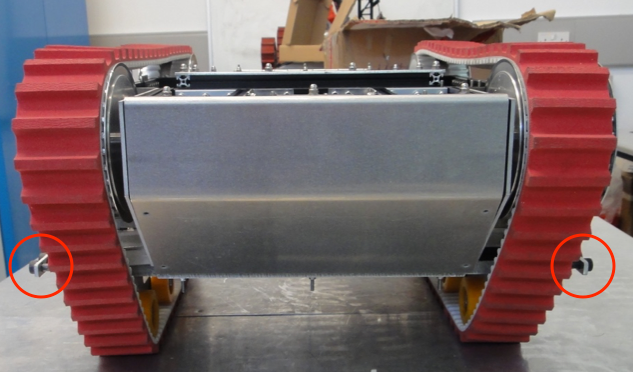
\includegraphics[width=0.6\linewidth]{Images/MaxImages/OrionFront.png}
\caption{Exposed Suspension Mounting Hardware}
\label{fig:OrionFront}
\end{figure}

The design has 16 pivoting joints in total, all of which are wear surfaces and will require lubrication and maintenance. This is not ideal for an urban search and rescue robot which will operate in harsh environments where particulate matter may contaminate bearing surfaces. The bearings used were all small (4mm I.D, 5mm width) sealed cartridge ball-bearings, replacing these in a field situation would be a tedious task. Furthermore, as the bearings were small the bearing surface was also small. This meant that each bearing was subjected to a high load during testing and operation. This loading would likely cause premature wear and resistance of the suspension linkage, compromising performance.

Overall the design is complex and difficult the assemble. There are nine parts for each suspension assembly that must be aligned correctly and held in position to be threaded in to place. The mounting bolts must also be not be over-tightened to avoid bending the outer mounting plates and locking the suspension, further complicating in-field repairs. 

The coil spring design also lacks adjustability. The springs do have adjustable reload, however there is no mechanism for adjusting the spring rate or ground clearance of the vehicle without disassembling the whole suspension system, which is a time consuming and complex task. This means that the suspension cannot be levelled if there is uneven weight distribution of the robot.


A positive aspect of this coil-spring design is relatively low un-sprung mass and the damping built into the coil spring units. The damping was beneficial because it stops the suspension from oscillating between compression and extension following an impact, returning the suspension to the neutral position more quickly.

The suspension design could have been modified to improve the performance, for example mounting spacers to prevent the mounting plates from bending inwards and fouling the mounting bolts. The lack of sag could be addressed by moving the upper coil spring mounting points lower or replacing the coil springs for longer units, however this would further increase the height of the centre of gravity, which is not desirable. Overall, due to the limitations of the design and lack of robustness, a new suspension design was most appropriate, as the what was learnt from the shortcoming of the coil spring design could be used to create higher performance suspension more suited to the needs of the robot.

\subsubsection{Review of Possible Alternative Suspension Designs}
Several alternative suspension designs were considered to replace the current coil spring design. The alternatives were considered on function, manufacturability and weight. All alternatives would have to improve on the current design to be a realistic option.\par

The first option to be considered was removing the suspension entirely and fixing the idlers directly to the base plate of the robot. Such a design would the the simplest, lightest and most robust as there are no moving parts nor extra mechanisms needed. However, as explained in the section titled “Why Have Suspension” there are many benefits to having a form of suspension and it was thought that removing it would limit the capabilities of the robot. \par

A second option considered was modifying the current suspension to rectify some of the problems it has with components fouling each other and bending when tightened properly. This would have a lower design and manufacturing time than re-designing from scratch. It was decided however, that the time savings were not worth the significant drawback in the design, namely the complexity and fragility.\par

Traditional suspension designs for tracked vehicles were then reviewed and considered. A type of suspension that has been used for tracked vehicles is Christie suspension. It is comprised of a coil spring mounted horizontally which is actuated by a bell-crank \cite{Mastinu11}. Christie suspension provides a large range of motion but reduced the internal volume of the chassis \cite{Zaloga15}. To contain all the internal components of the robot it is not feasible to reduce the internal volume, so this design was disregarded. 
\par

The most widely used type is torsion bar suspension \cite{Mastinu11}. Torsion bar suspension uses a bar mounted to a swing arm to provide a spring action in torsion (Figure \ref{fig:torsionbar}). One end of the torsion bar is fixed to a swing-arm on which a road wheel is mounted and the other end is fixed to the hull of the vehicle \cite{Mastinu11}. \par
\begin{figure}[h]
\centering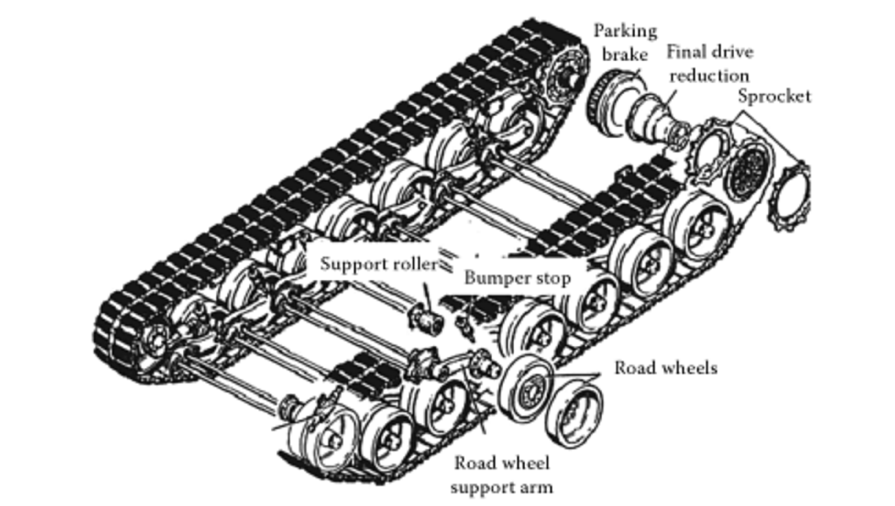
\includegraphics[width=0.6\linewidth]{Images/MaxImages/torsionbarsus.png}
\caption{Torsion Bar Suspension \cite{Mastinu11}}
\label{fig:torsionbar}
\end{figure}
The torsion bar design has been widely adopted because of its simplicity lightweight associated with this. Torsion bar suspension also stores more energy for the same weight than other systems do, further reducing weight \citet{Hohl85}. Torsion bars can be mounted inside the vehicle to project from damage or underneath the vehicle to increase interior volume, the second option would be suitable for the robot as maximum interior volume is needed to house the electronic components and the suspension should not protrude past the outside line of the tracks. Whilst the bars may be vulnerable to damage sitting outside the chassis the components are simple to replace \cite{Hohl85}. 

The spring rate of torsion bars can be changed by changing the the diameter of the bar or the length so it could be possible to include an adjustment mechanism in a design to change the spring rate and therefore the ride-height, allowing the robot to be levelled. Such adjustability would allow the pitch of the chassis to be changed depending on terrain conditions, improving tractive performance \cite{Wong88}. The shorter a torsion bar is the, stiffer and therefore the higher the spring rate.

\[ k = \frac{ \pi\times d^4 \times G}{32L} \]
\[k = spring\:rate\:(N/m), d = diameter\:(m), G = Young's\:modulus\:(N/m^2), L = length\:(m)\]

There are some disadvantages, however. Torsion bars do not self-damp \cite{Hohl85}, so either dampers will need to be included in the design or not used. Whilst not using dampers for a fast-moving tracked vehicle would be unfeasible the robot travel at a maximum speed of 0.5m/s and will weigh less than 25kg. Firstly, it is likely that the robot will be travelling too slowly for any large oscillations to be induced and secondly there will be a degree of coulomb (sliding friction) damping \cite{Persson00} in the suspension system, especially the dynamic tensioners which will feature steel rod sliding through an aluminium block in the direction opposite to suspension compression or extension. Secondly, the spring rate of torsion bars is linear, not progressive as coil springs are \cite{Hohl85}. For larger vehicles progressive spring rates are preferable, however it is an acceptable compromise in return for a robust and simple suspension system.

Overall it was deemed that the advantages of torsion bar suspension, namely; simplicity, light weight, robustness, the potential for adjustability, no reduction in internal volume and good packaging outweighed the disadvantages of no inherent damping and linear spring rate. 


\subsubsection{Design of Orion's Torsion Bar Suspension}
To summarise, torsion bar suspension was chosen for the following reasons in Table 1. These reasons formed the basis of the suspension requirements. The suspension design must fulfil these requirements.
\begin{table}[h]
\centering
\begin{tabular}{l}
\hline
Good performance\\
No internal volume lost\\
Adjustable\\
Robust\\
Simple\\
Easy to manufacture\\
Low external profile\\
\hline
\end{tabular}
\caption{Reasons for Torsion Bar Suspension}
\end{table}

When designing the torsion bar suspension, it was a priority to keep all parts as simple as possible. Reducing complexity makes the design and manufacturing phases shorter, improves the reliability of a design and takes in-service maintenance and repair simpler. The current suspension was analysed to determine which components could be reused. It was decided to reuse the idlers from the previous design and well at retain the same swing arm length of 80mm \par

Suspension design was started by calculating the dimensions of the components critical to the function of the suspension. Firstly, the amount of suspension travel needed to be decided. The previous design had a total spring travel of 25mm, allowing a maximum compression of 12mm, as spring are not recommended to compress more than half of their travel. There is no maximum travel of torsion bar suspension. As long as the shear stress in the torsion bar does not exceed the shear modulus of the material the suspension will continue to function. It was decided that a reasonable twist angle under maximum compression (dropping the robot from 350mm) was 20° (0.35rad) from the starting position to the horizontal. This gave approximately 27mm, 2.25 times the travel of Orion. The suspension was able to rotate a further 5.7° (0.1rad) past the horizontal before bottoming out. This zone is not intended for normal operation and is there to prevent the suspension from running out of travel and contracting the shell.\par

\begin{equation}
T= sin(\theta) \times L
\end{equation}

\[T = sin(0.35) \times 80 = 27mm\]


Figure \ref{fig:SwingDiag} shows the path of the swing-arm under compression. The swing-arm starts at “S”, the neutral position and can be compressed normally to anywhere in the zone marked by the green dotted line. The swing angle (Θ$_1$ ) in this zone is 20° (0.35rad). The zone marked by the red dotted line is the extra travel which is not meant to be used but guards against the swing-arm from contacting the chassis during compression. The swing angle (Θ$_2$ ) in this zone is 5.7° (0.1rad).

\begin{figure}[h]
\centering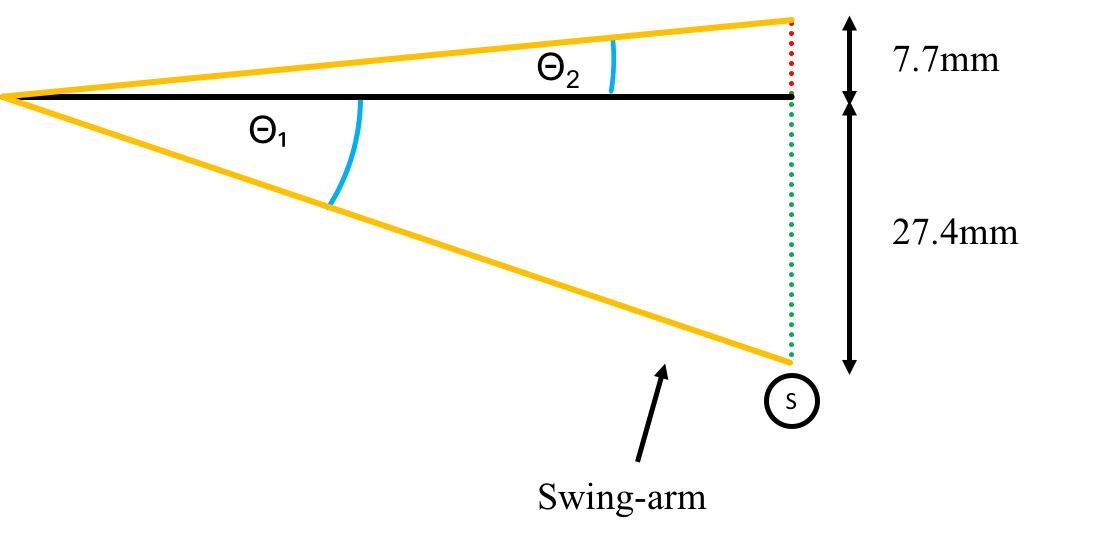
\includegraphics[width=0.6\linewidth]{Images/MaxImages/Swing_Diag.png}
\caption{Suspension Compression Path}
\label{fig:SwingDiag}
\end{figure}

Another consideration of travel is ground clearance and centre of gravity. The centre of gravity of Orion 2014 was relatively high \textcolor{red}{(prove this)}and it was felt that the robot did not need as much clearance.\par SAY SOMETHING

Having determined the length of the swing-arm and the swing angle for the travel needed when dropped from 350mm the force of this drop was calculated given a robot weight of 25kg. The force was calculated to be 738N (3 S.F) per corner, giving a torque on the torsion bar of 62.7N (3 S.F).\par
\begin{equation}
 F = \frac{m \times g \times h}{stopping\:distance} = \frac{25 \times 9.81 \times 0.35}{0.0274} = 3132.775N
\end{equation}

\[\frac{3132.775}{4} = 783.189N \approx 783N\]

\begin{equation}
T = F \times d\ = 783.189 \times 0.08 = 62.655Nm
\end{equation}

The polar moment of inertia of a torsion bar of a given cross-section was calculated as well as the length of bar needed to allow a 20°m swing angle for three materials of bar (magnesium, aluminium and steel). The sections considered were cylindrical and rectangular The dimensions of the torsion bar and blade were modified in an Excel model to give a suitable length of bar that would allow good adjustability. 

\begin{equation}
Circular\:section: J = \frac{\pi(d^4)}{32}
\end{equation}

\[J = \frac{\pi(0.006)^4}{32} = 12.72\times 10^{-11}m^4\]

\begin{equation}
Rectangular\: section: J = \frac{bh}{12}(b^2 + h^2)
\end{equation}


\[J = \frac{0.00635\times0.002}{12}(0.00635^2 + 0.002^2) = 4.69\times10^{-11}m^4\]

The minimum maximum length of torsion bar needed to absorb a fall from 350mm if the robot were to weight 25kg was calculated. The overall width of the robot was to remain the same, therefore the maximum length of the torsion bars was 119mm, leaving a 10mm gap between the left- and right-hand bars. Subtracting material thicknesses gave an adjustable range of 99mm. Torsion bar lengths were calculated for all materials. The results showed that the most suitable material for a torsion bar was 6mm diameter aluminium, needing a length of 49.0mm to absorb the fall; a steel torsion blade (6.35mm by 2mm) needed to be 52.4mm. Both lengths give a wide range of adjustability in the 99mm maximum length, allowing the suspension to be softened and lowered or stiffened and raised as needed.\par

\begin{equation}
Length = \frac{\theta(J \times G)}{T}
\end{equation}

\[\theta = Twist\:angle\:(radians), J = polar\:moment\:of\:inertia (m^4),\]
\[G = Young's\:modulus (N/m^2), T = Torque (Nm)\]

\[Aluminium\:bar: L = \frac{0.35(12.72\times 10^{-11} \times 45 \times 10^{-9})}{62.64}\]
\[L = 0.0490m = 49.0mm\]

\[Steel\:blade: L = \frac{0.35(4.69\times10^{-11} \times 200 \times 10^{9})}{62.64}\]
\[L = 0.0524m = 52.4mm\]
The steel blade was more suitable because of the higher sheer modulus of steel (79GPa) against aluminium (25.5GPa) (Crandall78), which is critical as the torsion bars will experience significant shear force. Furthermore, from a manufacturability standpoint it would be easier to fix a flat blade to other component than a cylindrical bar. Using a steel torsion bar was investigated but found to be unfeasible due to the small diameter required for a good range of adjustability.

Spring rate was calculated to determine the spring rate of needed for the dynamic tensioning system. The spring rate of all materials and their respective lengths was the same as they all had to absorb the energy from the drop, therefore the spring rate was calculated using the data for the 6mm aluminium bar, as is simplified calculations.

\begin{equation}
Spring\:rate = \frac{\pi \times d^4 \times G}{34L}
\end{equation}

\[Spring\: rate = \frac{\pi \times 0.006^2 \times 45\times10^{9}}{34\times 0.00490} = 179.0 N/m\]

A rail system with a movable anchor point for the torsion blade was designed to allow the effective length to be varied to adjust spring rate and therefore travel and ground clearance. The rail system would be made from MakerBeam. There were concerns that the “wings” of the MakerBeam would not withstand the tensile and compressive forces subjected to the suspension during compression. A simulation was run on on the MakerBeam rails (Figure \ref{fig:SuspensionSim3}), subjecting one side to tensile stress and the other to compressive stress, as would happen when the suspension is compressed and the blade under torsion, which is then transferred to the baseplate via the MakerBeam. The tensile and compressive loads simulated were 10000N, significantly higher than the robot would see under normal operation. The MakerBeam plastically deformed by approximately 0.01mm and is subjected to stress of \textcolor{red}{INSERT INFO HERE}.

\begin{figure}[h]
\centering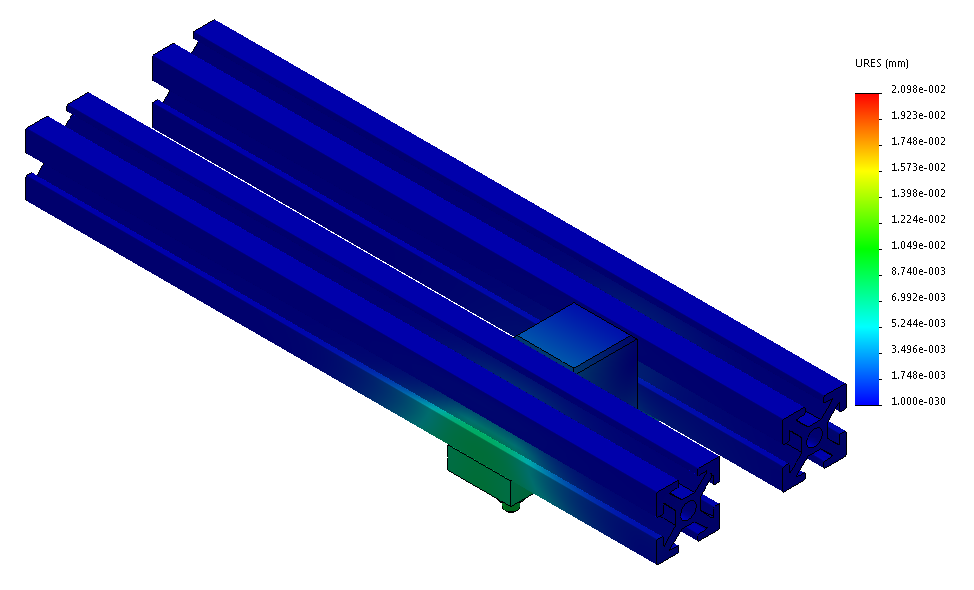
\includegraphics[width=0.6\linewidth]{Images/MaxImages/Suspension_beam_sim_3.png}
\caption{MakerBeam Rail Deformation}
\label{fig:SuspensionSim3}
\end{figure}
The machine screws fixing the tuning block to the MakerBeam was subjected to approximately 380MPa under the applied loads. The yield stress of an M2.5 scews is 1300MPa (Viewmold16), therefore the stress that will be exerted on the screws during normal operation will not exceed the yield stress of the fixings. This is shown in Figure \ref{fig:SuspensionSim1}.
\begin{figure}[h]
\centering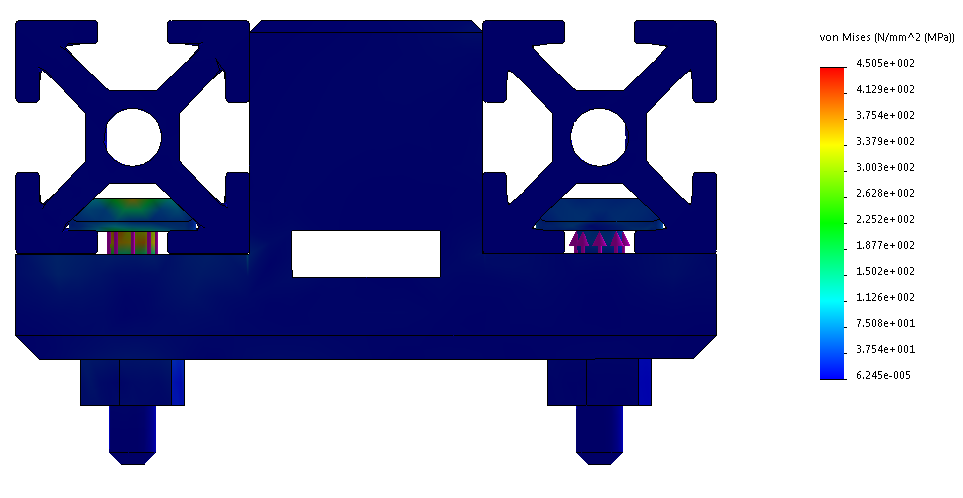
\includegraphics[width=0.6\linewidth]{Images/MaxImages/Suspension_beam_sim_1.png}
\caption{Stress on MakerBeam Fixings}
\label{fig:SuspensionSim1}
\end{figure}
Where possible components were designed to be as close to stock material sizes as possible to reduce manufacturing time. An example of this are the swing-arms. The first design used a heavily contoured part that would have to be CNC machined. The set-up of this process would have been time consuming due to the intricacy of the design. The swing-arm was redesigned to make manufactured from a stock U-section. The aluminium extrusion would be stiffer than previous design and simpler to manufacture. The section could be cut to length and the appropriate holes drilled with no significant machining required. 

INSERT IMAGES OF BOTH SAs

2014/2015’s Orion used 8 small sealed ball-bearing cartridges (4mm I.D, 5mm width) through which all the impact force from the terrain was transferred into the chassis. To improve on this polymer plain bearings were used, again 8, however width was 10mm, providing double the bearing surface. A second advantage of was that the polymer will not corrode, unlike the previous steel bearings. The robot could operate in harsh environmental conditions making corrosion resistance a consideration.

The torsion bar suspension set-up fitted to Cyclone was designed using the lessons learnt form Orion as guidance. The problems highlighted in the critical analysis of the suspension are all problems which could disable the robot in the field and the new design sought to address theses. The torsion bar suspension, while undamped, did address the issues of the coil spring design and would provide a more robust system that is also simpler. Table \ref{fig:SusComp} compares the suspension systems of Orion and Cyclone.

\begin{table}[h]
\centering
\begin{tabular}{l l l}
\hline
\textbf{} & \textbf{Orion 2014} & \textbf{Orion 2016}\\
\hline
Travel & 12mm & 27mm\\
Ground Clearance & 100mm & 93mm \\
Adjustability & Fixed travel \& ground clearance&  Adjustable travel \& ground clearance\\
Pivot Points & 16 & 8\\
Parts Count & 16 & 16\\
\hline
\end{tabular}
\caption{Comparison of Orion's and Cyclone's Suspension}
\label{fig:SusComp}
\end{table}

\subsubsection{Simulation of Suspension Components}

To assist the design and validation of the suspension components stress simulations were carried out. The service conditions of the components were known and were used to form the basis of the simulations. If the components exceeded the materials yield strength or did not perform satisfactorily the design, dimensions or materials were changed.

\paragraph{Blade Adapter}

Figure \ref{fig:BladeAdapterSim} is a simulation applying 783N (the calculated force on one suspension assembly when dropped from 350mm) in the Y-axis to the smaller diameter section of the blade adapter. This simulated what would happen if the torsion blades were set far too short and not allowed to function as springs. This would transfer all of drop force into the blade adapter. From the image it is clear that the maximum stress (134.9MPa) is lower than the yield stresses of 6063-T6 aluminium (215MPa) (Davis93) and silver steel (640MPa) (Smith94). The decision was made to manufacture the component from silver steel as it allows a greater factor of safety as well as a better bearing surface when compared to aluminium. Furthermore, the average stress on the blade adapter is 50MPa, 5x lower than the yield stress of silver steel.

\begin{figure}[h]
\centering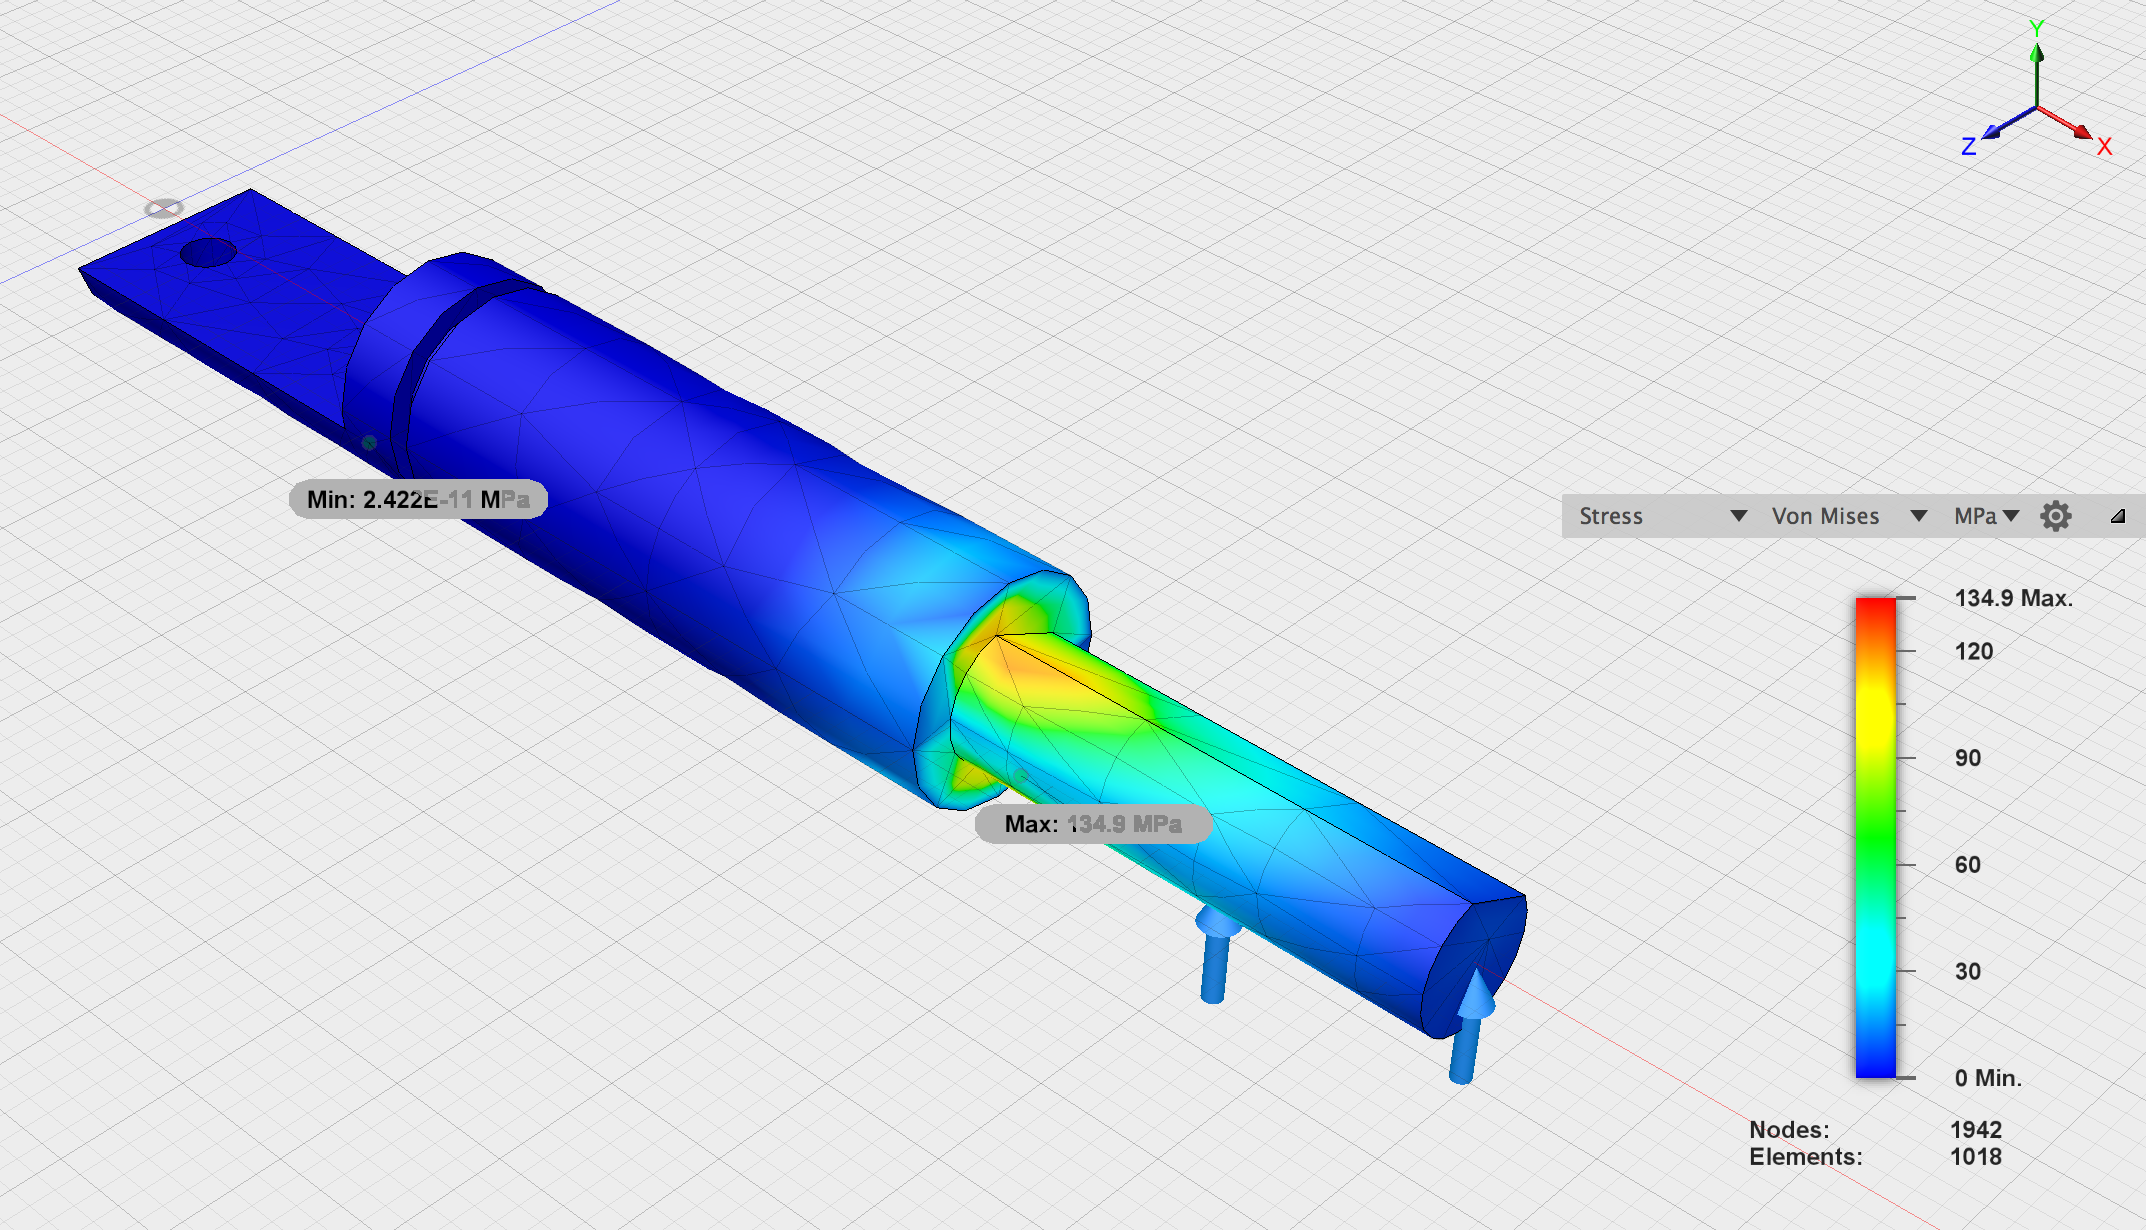
\includegraphics[width=0.6\linewidth]{Images/MaxImages/BladeAdapterSim.png}
\caption{Simulation of the Blade Adapter}
\label{fig:BladeAdapterSim}
\end{figure}

\paragraph{Torsion Blade and Blade Adapter}

Simulations investigating the shear stress on the torsion blade and  blade adapter were also run. When a torque of 62.64 Nm (the torque when dropped from 350mm) is applied to the blade adapter the maximum shear stress on blade adapter is 4042MPa (4.042GPa), the minimum stress is -7237MPa (-7.237GPa), which can be treated as 7237MPa (7.237GPa). The shear modulus of steel is 79GPa (Crandall78), giving a factor of safety of over 10x. The average shear stress on the blade adapter is around 80MPa (0.08GPa) and around 1800MPa (1.8GPa) on the torsion blade, as seen in Figure \ref{fig:TorsionBladeandAdapter}, and will therefore have an even greater factor of safety. This means that during normal operation the shear stresses exerted on the blade adapter and torsion blade will not cause the components to plastically deform.

\begin{figure}[h]
\centering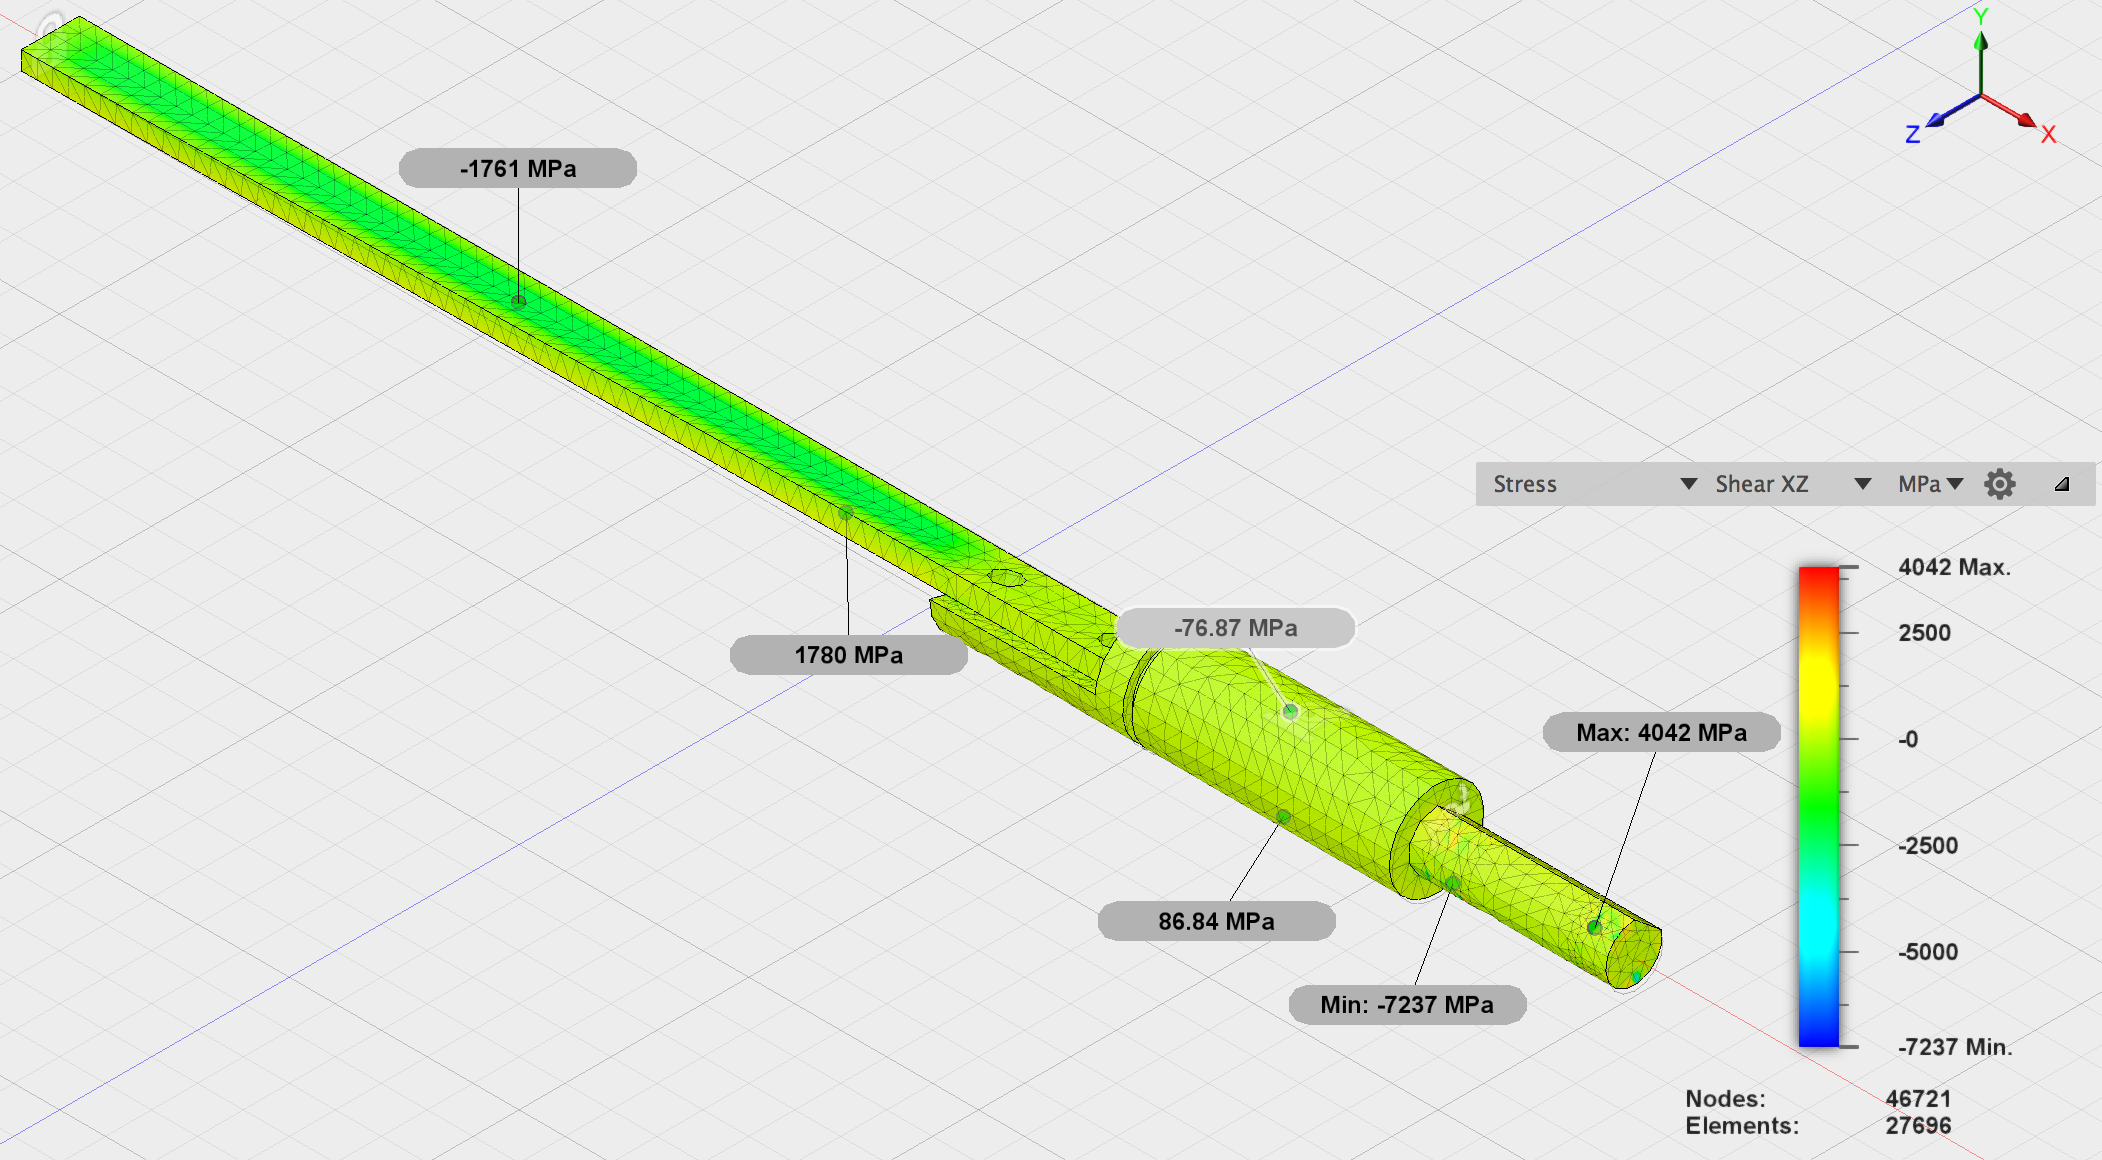
\includegraphics[width=0.6\linewidth]{Images/MaxImages/TorsionBladeandAdapter.png}
\caption{Simulation of the Torsion Blade and Blade Adapter}
\label{fig:TorsionBladeandAdapter}
\end{figure}
%\subsection{Dynamic Tension System}
\subsubsection{What is a Dynamic Tension System?}
The dynamic tension system is contained within the front module of Cyclone and ensures that changes in the track tension due to the motion of the suspension are sufficiently counteracted. This  avoids failure due to track derailment. Each track’s tension is independently controlled which is imperative for crossing rough, uneven terrain. \par
Each system consists of a pillow block, two springs, two rods and four spring caps. The front axles, onto which the wheels are fixed, are then placed through the pillow blocks to complete the dynamic tension system seen in figure \ref{fig:DTEN}. The system is held in place by linear bearings which are bolted to the bulkhead, connecting the front module to the centre module. The rods, which are inside the springs, pass through these bearings and are then able to move freely, in a linear motion to enable the system to perform its functionality of providing tension to the tracks. The system is installed in such a way that it will work in conjunction with, but in a reverse manner to  the suspension. When the suspension is compressed, the dynamic tensioning springs will extend to remove the slack produced, by pushing the axle forward, and vice versa. This system will lower the risk of track failure whilst the robot is in operation and thus avoid the manual collection of Cyclone by rescue personnel from potentially hazardous environments. \par
\begin{figure}[h]
\centering\includegraphics[width=0.8\linewidth]{Images/DTEN_render_1_spring.png}
\caption{Cyclone's Dynamic Tension System Assembly}
\label{fig:DTEN}
\end{figure}
\subsubsection{Analysis of Orion's System}
Orion (2014/15 WMR robot) used a static tensioning system  to alter the tension in the tracks by means of an adapted screw used to locate the pillow blocks in order to tension the tracks. Although simplistic and therefore easy to design and implement, the static nature of this design means that it is not practical for it’s intended purpose (to tension the tracks whilst in motion). During operation, if Orion’s suspension contracted in order to traverse an uneven surface, there would be a high risk of the tracks derailing from the wheels as there is no system in place to reduce this slack whilst the robot is in motion. \par
\subsubsection{Design for Cyclone's System}
As aforementioned, Cyclone will use a dynamic tensioning system. The decision was made to adapt the static system from the previous design to allow dynamic functionality. This allows for the reuse of many of the original components from the previous years design, keeping the design simple and saving on time for both design and manufacture. Springs were chosen as the method of applying a force to the pillow blocks to push the front axles forward so to tension the tracks.  This was found to be the simplest way to provide a force and is easy to implement into the design adapted from the previous year. \par
In order to fully adapt the previous design to that of Cyclones, its faults had to be corrected. This was namely the poor selection of bearings. The linear bearings in the pillow blocks of Orion were replaced with rotational bearings more suited to the rotational motion of the axles. Linear bearings were also used in the bulkhead to allow for the smooth movement of the rods. \par
During design, it was discovered that there was the risk of beaching if the dynamic tensioning system contracted too far, therefore exposing the frame of the robot (ADD FIGURE). To avoid this, the frame was altered to give a shallower profile and a simple stopper was installed in the front module to prevent the springs from contracting too far. \par
IMAGES OF THE BEACHING AND CORRECTIONS. \par
In order to decipher which type of spring was required, specifications had to be identified. The main requirement is that the total spring rate of the systems must not be larger than that of the suspension so that they are not preventing the suspension from performing its own function. Therefore, the spring rate for each of the four springs (two per track) needed to be less than 0.1829 N/mm since this is the value calculated from the suspension. The second requirement is that the springs should allow for the same amount of travel as the suspension to ensure the track tension does not suffer as a result. The maximum travel for the suspension is calculated to be 34mm, and therefore the travel of the dynamic tensioning systems will be at least 34mm. It was advised by the manufacturers that the springs must not be compressed by greater than 80\% of its total length for a continuous period as this will affect its performance. Due to the confined space within which the dynamic tensioning system is located, the free length of the springs is also a factor, this length is limited to 64mm as seen in (ADD IMAGE). The springs also require an inner diameter larger than 10mm (the rod diameter). \par
There was a limited availability of springs that fit these requirements. However, after consultation with Lee Spring, two different types of spring were chosen, seen in table \ref{tab:springparas}. This allowed for testing of both springs and ultimately the (WHICH SPRING WAS CHOSEN?) spring was chosen for the dynamic tensioning. \par
\begin{table}[h]
\centering
\begin{tabular}{|c|c|c|}
\hline
& \multicolumn{2}{|c|}{\textbf{Spring Type}} \\
\hline
Parameters & LP 032K 06 S316 & LP 029K 06 S316 \\
\hline
Outside Diameter (mm) & 13.716 & 13.716 \\
Inside Diameter (mm) & 12.904 & 12.980 \\
Wire Diameter (mm) & 0.812 & 0.736 \\
Free Length (mm) & 50.800 & 50.800 \\
Closed Length (mm) & 10.718 & 8.737 \\
Recommended Travel (mm) & 32.066 & 33.650 \\
Spring Rate (N/mm) & 0.170 & 0.130 \\
\hline
\end{tabular}
\caption{Parameters of Spring Choices}
\label{tab:springparas}
\end{table}

%%% THINGS TO DO %%
% - EDIT ALL TABLES: SIZES, BOLD, ETC.. %
% - HOW TO MAKE A BOLD ROW %
% - ADD IN SOLDERED BATTMON BOARD %
% - ADD IN SOLDERED LED BOARD %

\subsection{Electronics}

%% SYSTEM OVERVIEW %%
\subsubsection{System Overview}
The electronics architecture has been improved from the design proposed by the WMR 2014/15 team.\par

\begin{figure}[ht]
\centering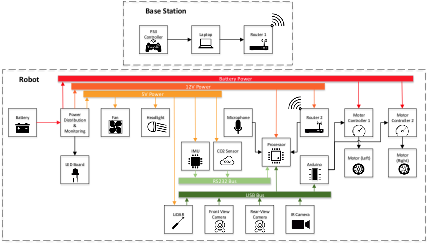
\includegraphics[width=0.8\linewidth]
{Images/ElectronicsFigures/ElectronicsBlockDiagram.png}
\caption{Electronics Systems Diagram}
\label{fig:eleoverview}
\end{figure}

The key differences include the addition of a second router at the base station. This approach has been implemented to overcome the ‘connectivity issues’ that many past WMR teams have experienced at the competition. The new router has superior performance over a laptops Wi-Fi card and so will improve the connectivity between the robot and the base station.\par

A second key difference is the removal of the bulky 8-to-1 USB splitter. This device limited the speed that the USB peripherals can run at, bottle-necking 8 data streams into 1, due to the maximum capable speed on USB 2.0. To ensure good quality video streams, it is proposed the RS232 ports of the robot's computer are utilised. Both the CO2 sensor and Inertial Measurement Unit (IMU) have compatible RS232 outputs.\par

It was discovered that a single threaded microcontroller could not reliably support the control of the motors whilst pseudo-simultaneously monitoring sub-systems. Therefore, a dedicated microcontroller is proposed for each motor, with the option to change this to a multi-threaded device in the future should additional sensors be required.\par

The final distinct difference regards the rationalisation of the power distribution and battery monitoring board from two separate entities into one, plus the addition of a dedicated LED board.\par

%% PROCESSOR %%
\subsubsection{Processor}
A quintessential component within the robot is the processor board. This board runs the Ubuntu OS and the ROS master software, so is responsible for managing each of the subsystems simultaneously, whilst maintain a live feed of information to the base station laptop. A range of processor boards were considered and the results against the requirement criteria are given in Table \ref{tab:procomp}.\par

% MAKE SOME ROWS/COLUMNS BOLD? %
\begin{table}[ht]
\resizebox{\linewidth}{!}{
\begin{tabular}{>{\bfseries}c c s s c s s s c }
\toprule
\multicolumn{1}{c}{}& & \multicolumn{2}{c}{Power Supply} & \multicolumn{3}{c}{Processing} & \multicolumn{2}{c}{I/O Capability} \\
\cline{3-9}
 & Dimensions& Voltage & Power & & Speed & DDR3 & & \\
Processor Board & (mm) & (V) & (W) & Chipset & (GHz) & (GB) & USB & Other\\
\hline
Axiotex PICO831 & 100 x 72 & 5 & 15 & Intel Atom N2800 & 1.86 & 4 & 4 & 2x RS232  \\ 
Intel NUC5i5MYBE & 115 x 111 & 19 & 65 & Intel Core i5 & 2,3 & 16 & 6 & -  \\ 
Axiotex PICO842 & 100 x 72 & 12 & 10,8 & Intel Celeron J1900 & 2,42 & 8 & 4 & 2x RS232 \\ 
\hline
\end{tabular}
}
\caption{Processor Comparison}
\label{tab:procomp}
\end{table}
%[REF1 - 3]

Last year's WMR team chose the PICO831 as the robot computer shown above. This board utilises an Intel Atom N2800 chipset released in 2011 [RFE4] and can only support 4GB of DDR3 RAM capability. However, Cyclone requires a greater amount of RAM to support multiple, real-time camera feeds, so alternative options were considered.\par

The Intel NUC board was a good choice as it outperforms the previous board with its capability to support 16GB RAM. In addition, its processor runs 23\% faster and has an additional 2 USB ports compared to Orion, this comes to the detriment of power with this board drawing over 4 times as much power as the previous design. It was decided therefore that the more recent, PICO842 board utilising the Intel Celeron J1900 released later in 2013, was the best option [REF5]. This processor coupled with the AX93283 I/O expansion board [REF6], with Gigabit Ethernet capability provides a fast processing platform at low power consumption, and so therefore was selected as the ideal choice for our robot application.\par

%% MOTORS %%
\subsubsection{Motors}
The WMR project team of 2014/15 set to use Maxon EC-4pole 323217 motors coupled with the Maxon ESCON P/N 409510 controllers. It was discovered that these motors were not suitable for our robot, as discussed in greater detail in [JOE’S SECTIONS]. Therefore, a new set of motors (plus gear head) that were capable of providing a greater torque were required. A second requirement was that the new motors are compatible with the existing controllers already purchased. Table \ref{tab:motcomp} provides a summary of the results from the motor investigation.\par

% MAKE SOME ROWS/COLUMNS BOLD? %
\begin{table}[ht]
\centering
\resizebox{0.75\linewidth}{!}{
\begin{tabular}{>{\bfseries}c c c c c c c}
\hline
Option Number & Old & 1 & 2 & 3 & 4 & 5 \\ \hline
Motor & 323217 & 136203 & 136204 & 370356 & 305015 & 305015 \\ 
\hline
\hline
Efficiency  & 0.88 & 0.8 & 0.8 & 0.94 & 0.9 & 0.9 \\ \hline
Speed constant  & 907 & 579 & 445 & 102 & 346 & 346 \\ \hline
Speed/Torque constant  & 27.8 & 6.78 & 6.67 & 0.666 & 4.83 & 4.83 \\ \hline
Torque constant  & 0.0105 & 0.0165 & 0.0214 & 0.0934 & 0.0276 & 0.0276 \\ \hline
\  & \  & \  & \  & \  & \  & \  \\ \hline
Gear & 166945 & 203127 & 203127 & 223087 & 203127 & 326669 \\ 
\hline
\hline
Ratio & 122.8 & 126 & 126 & 26 & 126 & 123 \\ \hline
Efficiency & 0.7 & 0.72 & 0.72 & 0.83 & 0.72 & 0.7 \\ \hline
\  & \  & \  & \  & \  & \  & \  \\ \hline
Motor controller & 4094510 & 409510 & 409510 & 409510 & 409510 & 409510 \\ 
\hline
\hline
Efficiency & 0.98 & 0.98 & 0.98 & 0.98 & 0.98 & 0.98 \\ \hline
Voltage drop & 1 & 1 & 1 & 1 & 1 & 1 \\ \hline
\multicolumn{7}{c}{Results}  \\
\hline
\hline
No load (rpm) * & 77.938 & 45.341 & 34.847 & 52.431 & 30.482 & 30.358 \\ \hline
Incline (rpm)* & 74.06 & 44.419 & 33.941 & 51.992 & 29.825 & 29.685 \\ \hline
No load (A) & 0.899 & 0.596 & 0.46 & 0.377 & 0.317 & 0.334 \\ \hline
Incline (A)** & 10.278 & 6.817 & 5.256 & 4.309 & 3.623 & 3.817 \\ \hline
\end{tabular}
}
\caption{Motor Comparison}
\label{tab:motcomp}
\end{table}

* Speed at 18.5V, the theoretical minimum worse case scenario accounting for uneven cell discharge from the LiPo battery.\par
** Torque up an incline approximately 8Nm
[REF 1- 5 (motors)] [REF – 6-10 (Gear)] [REF 11 – Controller] JOE HAVE SAME REFERENCES?\par

The results show the theoretical speeds and current requirements for each of the motor/gear combinations. Mechanically the best motors are option 1, as they provide the most torque with option 5 providing the least torque. Conversely, from an electronics perspective, the power required to achieve those torques have almost the inverse relationship. Option 4 and 5 appear enticing due to their low power consumption, but this does come at a penalty on speed, which may be too slow for the robots operation.\par

Therefore, it was decided that to satisfy both mechanical and electronic requirements option 3 would be the motors of choice. The 94\% efficient DC 370356 motors coupled with the 83\% efficient 223087 gear head, are approximately 27\% more efficient than the old motors. This is important to help maximise the robot’s battery life.\par

%% MOTOR DRIVE PROCESSOR %%
\subsubsection{Motor Drive Processor}
The DC motors are managed via ESCON 50/50 P/N 409510 motor controllers. The motor velocity commands can be input by either an analogue or pulse-width-modulated (PWM) signal. Cyclone utilises the PWM functionality, as is boasts significant advantages particularly due to its insensitivity to noise. This trait is common across all digital signals, which has lead to their abundant usage in modern day electronics.\par

It was decided that the ATMega328 microcontroller on the Arduino Uno platform was suitable for this application. This cheap microcontroller is smaller and requires less power when compared to the Arduino Mega 2560 board; as proposed by the WMR 2014/15 team. In addition, an Arduino can be easily integrated with the ROS environment, plus software development is made easy with the intuitive Arduino IDE.\par

%% SENSOR ARRAY %%
\subsubsection{Sensor Array}
In order for the robot to compete at the RoboCup, it needs to be equipped with a range of sensors, and the greater the capability of the robot, the more points it will be awarded. It is for this reason that Cyclone’s architecture has been designed to handle a comprehensive range of sensors. Although the sensor arrays used in previous WMR builds are proven designs, a revision of these are required for Cyclone. The key reason for this is to take advantage of the latest cutting edge technology, whilst ensuring their compatibility with the ROS driven system within Cyclone. Table \ref{tab:sensarray} gives a summary of the sensors that will be used in Cyclone.\par

% MAKE SOME ROWS/COLUMNS BOLD? %
\begin{table}[ht]
\resizebox{\linewidth}{!}{
\begin{tabular}{c c c c c }
\hline
Sensor & \multicolumn{2}{c}{Part} & Own or Required & Interface  \\ \cline{2-3}
& Company & Part Number & & \\ \hline
LiDAR & Hokuyo & URG-04LX & Own & USB \\ \hline
IR Camera & Photon & 160 & Own & USB \\ \hline
Front-View Camera & - & - & Required & USB \\ \hline
Rear-View Camera & Microsoft & LifeCam HD-3000 & Own & USB \\ \hline
IMU & Xsens & MTi-28A53G35 & Own & RS232 \\ \hline
CO2 Sensor & DFR & SEN0159 & Own & RS232 \\ \hline
Microphone & - & - & Required & Microphone \\ \hline
Headlight & - & - & Required & - \\ \hline
\end{tabular}
}
\caption{Cyclones Sesnor Array}
\label{tab:sensarray}
\end{table}


%% BATTERY MONITOR BOARD - OVERVIEW %%
\subsubsection{Battery Monitor Board}
\paragraph{Overview}
The 2014/15 WMR team designed and manufactured a power distribution board. It was capable of providing regulated power at 12V or 5V to each robot subsystem. However, after a critical analysis of the board it was decided a redesign was needed for the following reasons:\par

\begin{enumerate}
\item When tested, the 12V regulator was not producing the required output. It would require major board modifications, which are not easy to do on buried PCB traces.
\item The 5V regulator was not appropriate for the design, due to over cautious estimations of its output power requirement. This meant it would operate at a much lower efficiency than expected. It would severely reduce the robots battery life and cause the regulator to get undesirably hot. 
\item The max current output from the 12V regulator was too small and it would not have been capable of powering the new processor board. 
\item There was no consideration for how battery monitoring and automatic shutdown of the robot could be implemented. Additionally, there was no consideration for how a master power switch and E-Stop button would be integrated. 
\item There were redundant current limiting fuses that would not have blown in the event of an over-current draw.
\item The design has neither an output to drive the motors or the raw battery voltage that may be required in the future design of an arm.
\end{enumerate}

%% BATTERY MONITORING - PRINCIPLE OPERATIONS %%
\paragraph{Principle Operations}
A new integrated battery distribution \& monitoring board was therefore designed, with the schematic given in [APPENDIX 1]. The robot utilises Lithium-Polymer (LiPo) batteries due to their compact size, large capacity and high discharge rate. These are volatile as they use dry electrolyte polymer sheets, which can burst or catch fire if mistreated [REF1]. So each of the batteries cells are monitored to ensure they stay within their safe operating conditions, whilst also ensuring their maximum power is drawn from them.\par

It is for this reason that an ATMega328 microcontroller is required on the board. It has 6x 10-bit ADC inputs, which are used to monitor each of the cells to an accuracy of 4.88mV. The microcontroller updates an LED array with the current battery voltage, in addition to sending messages back through ROS to display this level on the operators GUI. Not only this, but should the warnings be ignored, the microcontroller will automatically shut down the entire robot, to ensure the safety and longevity of the battery.\par

An additional safety feature this microcontroller handles is the monitoring of sub-systems ‘heartbeats’. The electronic systems output periodic pulses when operating correctly, which can be monitored. In the event of a software glitch, the ‘heartbeat’ is not received, and the operation of the robot is likely to be unknown and uncontrollable; this also causes the controller to shut down the robot, as a precaution. The battery status LED would begin to flash at an identifiable frequency, so that the reason for the shutdown is known.\par

Some additional hardware safety features have also been incorporated into the design. An emergency stop and master power on/off switch have been included like many previous successful WMR designs. These switches had to be selected carefully to ensure they fulfilled the power requirements of Cyclone.\par

%% BATTERY MONITORING - VOLTAGE REGULATORS %%
\paragraph{Voltage Regulators}
The design team from last year had to make conservative estimations on the power drawn from each device. These values accounted for the worse case scenario and in cases were poor estimations of the true power drawn. Table \ref{tab:pwrreq} gives the updated power requirements of each of the devices. Note that to improve the accuracy of the results, some components have been measured using the actually device connected to a bench power supply.\par

% MAKE SOME ROWS/COLUMNS BOLD? %
\begin{table}[ht]
\resizebox{\linewidth}{!}{
\begin{tabular}{c c c c}
\hline
Device & Voltage (V) & Max Current (A) & Safety Margin  (+20\%) (A) \\ 
\hline
\hline
Motor (x2) & Battery & 8.6 & 10.32 \\ \hline
Motor Controllers (x2) & Battery & 0.172 & 0.2064 \\ \hline
\multicolumn{3}{r}{Total} & 10.5264 \\ 
\hline
\hline
Processor & 12 & 0.9 & 1.08 \\ \hline
Arduino (Motors) & 12 & 0.1 & 0.12 \\ \hline
Front Camera & 12 & 0.5 & 0.6 \\ \hline
Rear-View Camera & 12 & 0.5 & 0.6 \\ \hline
IR Camera & 12 & 0.5 & 0.6 \\ \hline
\multicolumn{3}{r}{Total} & 4.2 \\ 
\hline
\hline
Router & 12 & 1 & 1.2 \\ \hline
LiDAR & 5 & 0.5 & 0.6 \\ \hline
IMU & 5 & 0.07 & 0.084 \\ \hline
CO2 Sensor & 5 & 0.2 & 0.24 \\ \hline
Headlight & 5 & 0.35 & 0.42 \\ \hline
Fan & 5 & 0.236 & 0.2832 \\ \hline
\multicolumn{3}{r}{Total} & 1.6272 \\ 
\hline
\hline
\end{tabular}
}
\caption{Cyclones Power Requirements}
\label{tab:pwrreq}
\end{table}
%  [REF – ALL DATASHEETS?] %

A change in processor board coupled with these conservative estimates meant, the 5V regulator was overestimated and the 12V regulator was underestimated. Table \ref{tab:pwrreq} shows that the 1.63A and 4.20A are required from the 5V and 12V regulators respectively. The GE EHHD024A0A41 could supply 24A and the TRACO TEL30-2412 could provide a 2.5A output [REF2,3]. Figure \ref{fig:old5vg} shows an extracts from the GE EHHD024A0A41 datasheet.\par

\begin{figure}[ht]
\centering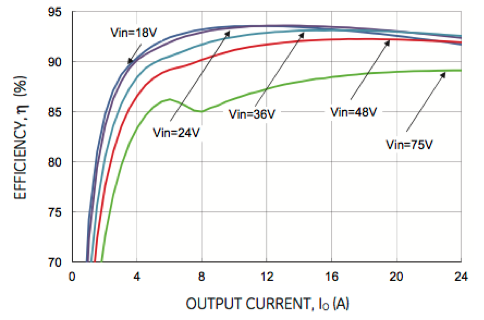
\includegraphics[width=0.8\linewidth]
{Images/ElectronicsFigures/RegulatorsGraph.png}
\caption{GE EHHD024A0A41 Efficiency against Output Current}
\label{fig:old5vg}
\end{figure}

This extract shows that at Cyclones expected current draw, this regulator would only be operating at around 70\% efficiency. So for these reasons a new set of regulators was considered. Table \ref{tab:regcomp} shows a comparison between the old and new components.\par

% MAKE SOME ROWS/COLUMNS BOLD? %
\begin{table}[ht]
\resizebox{\linewidth}{!}{
\begin{tabular}{c c c c c}
\hline
Part & Output Voltage (V) & Max Output Current (A) & Dimensions & Efficiency  \\ 
\hline
\hline
\multicolumn{5}{c}{WMR Power Distribution Board 2014/15} \\ \hline
TRACO TEL30-2412 & 12 & 2.5 & 2” x 1” & 0.91 \\ \hline
GE EHHD024A0A41 & 5 & 24 & 2.3” x 0.9” & \~70\% \\ \hline
\multicolumn{5}{c}{WMR Power Distribution Board 2015/16} \\ \hline
TRACO TEN60-2412N & 12 & 5 & 2” x 1” & 0.92 \\ \hline
TRACO TEN40-2411N & 5 & 8 & 2” x 1” & 0.91 \\ \hline
\end{tabular}
}
\caption{Regulators Comparison between Orion and Cyclone}
\label{tab:regcomp}
\end{table}
% [REF – 2,3,4,5] %


The TRACO TEN60-2412N and TRACO TEN40-2411N have been selected due to their high efficiency and small footprints. These rugged regulators satisfy the temperature requirements of the board with a wide operating range of \SI{-40}{\degree}C to \SI{+80}{\degree}C. Their maximum current outputs are greater than those calculated in Table \ref{tab:pwrreq}, but this is to allow for future expansion, with the inclusion of a robot arm.\par

\paragraph{Current Protection}
An over-current protection fuse has been incorporated into the design. The 25A Littelfuse was selected, such that if the current draw exceeded the expected maximum, allowing for a 20\% margin, then it would blow cutting the power to the robot.\par

\paragraph{Connectors}
This design requires many types of connectors, due to the number of mixed signal utilised in the design. All the connectors used within the robot were sourced from WMR sponsor, Harwin. Table \ref{tab:connectors} lists the selected connectors and identifies how they meet their associated requirements.\par

% MAKE SOME ROWS/COLUMNS BOLD? %
\begin{table}[ht]
\resizebox{\linewidth}{!}{
\begin{tabular}{c c c c c}
\hline
Purpose & Part Number & Gender & Quantity & Reason for Selection \\ \hline
Power & M80-5000000M2-02-331-00-000 & Male & 16 & Max current 20A per pin \\ \hline
Power & M80-4000000F1-02-325-00-000 & Female & 16 & Mating half \\ \hline
Heartbeat & M80-8810245 & Male & 2 & Friction Latches  \\ \hline
Heartbeat & M80-8990205 & Female & 2 & Mating half \\ \hline
LED Board & M80-8630842 & Male & 2 & Friction Latches \\ \hline
LED Board & M80-8890805 & Female & 2 & Mating half \\ \hline
Battery Mon & M80-8631042 & Male & 1 & Friction Latches \\ \hline
Battery Mon & M80-8891005 & Female & 1 & Mating half \\ \hline
USB Board & M20-9710645 & Male & 1 & Compatible pin pitch to USB board \\ \hline
\end{tabular}
}
\caption{Harwin Connectors Used on Cyclones Battery Monitoring \& Distribution Board}
\label{tab:connectors}
\end{table}
% [REF 1-9] %

Harwin’s MixTek range of connectors can support up to 20A of current through each pin so will suffice the power distribution operations. Conversely, It was decided that their L-Tek range was suitable for all the low power signals. All of the connectors listed contain either, a screw terminal lock in or a friction latch (12-14N of force). These were selected to ensure a reliable connection, even under the shock and vibration conditions the robot will be subject to at the competition.\par

\paragraph{Trace Sizings}
The track widths on the board needed to be sized to suffice the power requirements previously stated. The trace sizings calculated in Table \ref{tab:tracesize} are based on the worse case scenario using the IPC-2221 standard [REF1].\par

% MAKE SOME ROWS/COLUMNS BOLD? %
\begin{table}[ht]
\resizebox{\linewidth}{!}{
\begin{tabular}{ c c c c }
\hline
Trace & Max Current (with 20\% safety margin) (A) & Trace width Single-Sided (mm) & Trace width Double-Sided (mm) \\ \hline
Battery  & 13.78 & 7.35 & 3.68 \\ \hline
12V & 4.2 & 1.43 & 0.71 \\ \hline
5V & 1.63 & 0.39 & 0.19 \\ \hline
Signals & < 0.03 & Negligible & Not Necessary \\ \hline
\end{tabular}
}
\caption{Trace Sizings Required for each Power Line}
\label{tab:tracesize}
\end{table}

These sizings have been calculates on the standard trace thickness of 1$oz.ft^-2$ ($\approx$\SI{35}{\micro\meter}), allowing for a \SI{20}{\degree}C  rise of an external track when conducting; with an assumption of \SI{25}{\degree}C ambient temperature [REF2]. The board design utilises double sides traces to minimise trace width, with the plated through holes to electrically connect the two. It was decided that there were enough through-hole connections, such that resistance between the traces on each layer was negligible, so no additional ‘shorting‘ vias were required.\par

In addition, traces have been made as short as possible in order to reduce their resistance. A high parasitic resistance would lead to a voltage drop along the trace; this would introduce issues like a floating ground. Not to mention the power that will be lost, which is scarce within the robot. Traditionally, a multi-layer board is used to minimise these effects, but the additional cost and complexity is not required for this build.\par

\paragraph{Board Dimensions}
These considerations to minimise the amount of board real-estate were required to create a compact board that suffice the required mechanical dimensions. The central section of the robot is \SI{212 x 322 x 122}{\milli\meter}, so the board was sized to \SI{120 x 120}{\milli\meter}. Therefore, the board can be rearranged in many orientations, so that future teams could alter the arrangements if required. The Ultiboard layout is given in [FIGURE BELOW].\par

\begin{figure}[ht]
  \centering
  \begin{minipage}[b]{0.45\textwidth}
    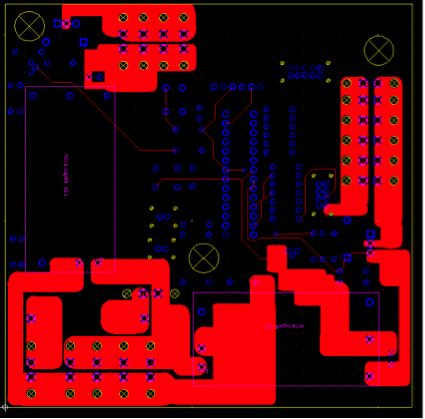
\includegraphics[width=\textwidth]{Images/ElectronicsFigures/BattMonBottom.png}
    \caption{Board Bottom-Side}
  \end{minipage}
  \hfill
  \begin{minipage}[b]{0.45\textwidth}
    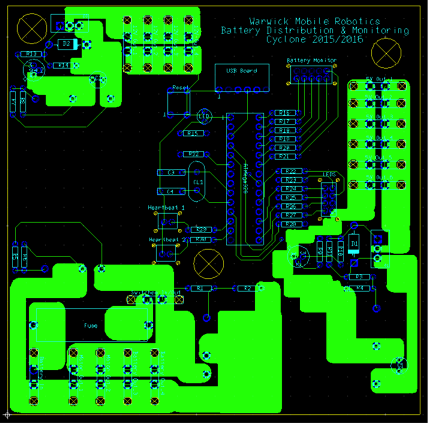
\includegraphics[width=\textwidth]{Images/ElectronicsFigures/BattMonTop.png}
    \caption{Board Top-Side}
  \end{minipage}
\end{figure}


\paragraph{Wire Sizings}
The wires carrying the current to and from the board also need to adhere to these power requirements. Table \ref{tab:wiresize} shows the wires thickness, in American Wire Gauge (AWG), selected from each part of the board [REF3].\par

% MAKE SOME ROWS/COLUMNS BOLD? %
\begin{table}[ht]
\resizebox{\linewidth}{!}{
\begin{tabular}{ c c c c }
\hline
Trace & Max Current (with 20\% safety margin) (A) & Wire Thickness (AWG) & Current Carrying Capability (A) \\ \hline
Battery  & 13.78 & 12 & 34 \\ \hline
12V & 4.2 & 14 & 24 \\ \hline
5V & 1.63 & 14 & 24 \\ \hline
Signals & < 0.03 & 22 & 5 \\ \hline
\end{tabular}
}
\caption{Wire Sizings Required for each Power Line}
\label{tab:wiresize}
\end{table}

\paragraph{Usability \& Testability}
A lot of thought went into the design to ensure maximum testability, plus the ability to modify the board if needed. In places, extra ‘dummy’ components where incorporated into the design with their pads laid out. However, the intention was to not fit these components, but have the ability to, should they be required during testing.\par

All components where selected to be through hole. This allowed ease of soldering and debugging of the board during testing. In addition, de-coupling capacitors where added to the outputs of the regulators. There purpose is to reduce the voltage ripple on their output, such that a smooth constant output is delivered to the remaining circuitry.\par

\paragraph{Component Placing}
Care was taken when placing the components in order to separate the high power ‘noisey’ circuitry, from the sensitive digital micro-controller circuits. In the designs layout, it was thought the regulators were placed on the backside of the board. The intention was these would be fixed to the robot casings, to aid with heat dissipation, whilst the connectors on the other side would still easily accessible to the rest of the sub-systems. However, there was a misinterpretation with the software and the regulators where not placed on the bottom of the board as expected.\par

\paragraph{Final Design}
The design was sent for manufacture at Euro circuits. They were selected as they could provide plated through holes, on a short-lead time, for at a reasonable price. The returned blank PCB was then populated with components, with the soldering done ‘in-house’ by hand, as shown in [FIGURE BELOW].\par

%% ADD SOLDERED PCB IMAGE - ON PHONE, CHNAGE REF ABOVE %%
% \begin{figure}[ht]
% \centering\includegraphics[width=0.8\linewidth]
% {Images/ElectronicsFigures/???.png}
% \caption{Battery Monitoring \& Distribution Board}
% \label{fig:finalboard}
% \end{figure}

\subsubsection{LED Board}
A second board was manufactured in the School of Engineering. This board consists of 6-power status LEDs and a robot status LED. This single sided board was design so that the LEDs can be placed externally from the previous board and can be made visible through the robot. All the routing is on a single-side of the board, however, the connector is orientation on the bottom side. This is so it can be connected on the inside of the robot, with the LEDs facing out of the robot. The 4 mounting holes allow the board to be fixed, with spacers to the robot using M3 screws.\par

%% ADD SOLDERED PCB IMAGE - ON PHONE, C %%
% \begin{figure}[ht]
% \centering\includegraphics[width=0.8\linewidth]
% {Images/ElectronicsFigures/???.png}
% \caption{LED Board}
% \label{fig:LEDboard}
% \end{figure}




%\section{Manufacturing}
%\subsection{Design For Manufacture}
\subsubsection{What is Design for Manufacture?}
Design for manufacture is part of Design for Manufacture and Assembly (DFMA). DFMA has three main aspects \cite{Boothroyd10}:

\begin{enumerate}
\item Form a foundation for concurrent engineering studies, providing direction to designers to simplify products to reduce the cost of manufacture and assembly and quantify improvements.
\item As a benchmarking tool to compare products for ease of both manufacturability and assembly.
\item As a “should-cost” tool for cost control and supplier negotiation.
\end{enumerate}
Firstly, concurrent engineering is a methodology that allows engineering effort to be integrated with the life cycle of a product and means that these efforts are carried out at the same time. This links upstream and downstream design processes and takes all stages of a product’s life-cycle into account from the outset \cite{Kusiak93}.

INSERT CONCURRENT ENDINEERING IMAGE


Design for manufacture takes into account the limitations of manufacturing processes as well as considers which processes, materials and techniques are best suited to produce a component most efficiently. Because of this it is critical that Design for Manufacture is used in the product life cycle as early as possible. In DFMA more time is spent in the early design stages (concept design) to establish the performance criteria and parameters. This reduces the design changes further into the product life cycle and reduces the time taken from product inception to market. DFMA can reduce to the time to market by up to 40\% \cite{Boothrody10}. Additionally, there should be more time spent on design in the early stages of the lifecycle because it is the decisions made here that dictate up to 70\% of the total costs. Intelligent and careful design is the greatest factor in reducing cost \cite{Boothroyd10}.

INSERT DMFA TIME SAVINGS IMAGE

\subsubsection{Concurrent Engineering and Design for Manufacture for Cyclone}
The use of concurrent engineering was appropriate to use because of the modular nature of the robot. The new design, the number modules needed and time constraints meant that design of the robot was split among group members to be carried out concurrently. This meant that during the design of each module, its interactions with the other modules had to be considered from the outset, to minimised changes that would have to be made later. Furthermore, because the WMR urban search and rescue project runs from year to year future changes and adaptations further into the robot’s life-cycle had to be taken into account. For example, a robotic arm should be added in the future meaning that the chassis had to be designed to be stiff and strong enough allow an arm to be mounted to the upper chassis. The suspension was also designed to be capable of functioning with the added weight of an arm, hence its adjustability. The motors were also capable of more torque than strictly needed to account for future weight increases and the circuit boards and control systems capable of running additional sensor and cameras in the future.

Cyclone is almost a brand new robot, very few parts were carried over from Orion of 2015. As a result of this there were many new parts designed and all of these would have to be manufactured. The number of parts that needed to be made meant that there were many opportunities for error and delay, which could set the project back and create problems further into the project, for example at assembly if parts have been made to different specifications. To limit the number of issues that would be encountered throughout the course of the project Design for Manufacture was employed to simplify both the design process, as well as manufacture. This would in turn reduce the overall project costs and also feed into Design for Assembly (Section XX).

There are a number of principles of Design for Manufacture, as described by \cite{Chang05}, some of these were used during the design of Cyclone. How these principles were applied to Cyclone is explained below (TOO CLUNKY):

\begin{enumerate}
\item \textit{Reduce total number of parts.}
\par The majority of parts reduction has come from changing the chassis from Makerbeam to plate aluminium. Orion had over 20 Makerbeam sections to make up just the central chassis section and far more fixings. Cyclone has 5 plates making the central chassis section and XX bolts. The situation is the same for the front and drive sections. The reduction in parts count reduces complexity greatly and made design easier as there were fewer part interactions to consider.
\item \textit{Develop a Modular Design}
\par The robot has a modular design. It is made up of three modules: front, mid and drive. These are connected to each other with 6 bolts. The benefit of the modular design is that the robot can be upgraded over time by swapping modules for new ones, or by removing a module to change its components. For example, the front module could be changed for one with a different set of sensors, for use under different conditions. Furthermore, modularity improves the ease or repair and fault finding, as a module can be quickly removed and all components easily accessed. To allow modularity, all connectors between the modules are standardised and located in one connector plate, allowing them to be quickly connected.
\item \textit{Use Standard Components}
\par The most distinct advantages of standard components are the cost and time benefits. Standard components can be bought off the shelf and do not require extensive engineering effort, allowing focus to be on other areas. There are several example of standard components in Cyclone. The linear bearings used in the dynamic tensioning system are stock parts from Igus bearings, which have simply been machined down to fit the packaging requirements. Another example is the suspension swing-arms; these could have been machined from a billed to a complex design but a using stock channel section meets the requirements but is vastly quicker to manufacture.
\item \textit{Design Parts to be Multifunctional}
\par By designing parts to be multifunctional the parts count and complexity of the robot could be reduced. An example of this is using the chassis itself as a heat-sink. Electronic components, such as the motor controllers, were positioned against large surfaces of the chassis to draw away heat and dissipate it though the chassis to the environment. Another example of this is chassis serving as the mounting points for the motors, rather than having motor mounts fixed to the chassis. The suspension’s primary purpose is to absorb bumps and shocks that the robot is subjected to, to allow it to traverse terrain more quickly and it also protects the robot from damage that uneven terrain could cause.
\item \textit{Design for Ease of Fabrication}
\par All parts have been designed to be as easy to manufacture as possible. As part of this, the majority of parts can be manufactured from one side. This means that fixturing during manufacturing is easy, as the parts to not need to be turned and repositioned, which could cause misalignment. Parts have been designed with stock material size in mind to reduce manufacturing time where possible. Examples of this are the drive shafts, which are 16mm meaning that they do not need to be turned down, only cut to length and additional features added, if needed.
\end{enumerate}
To summarise concurrent engineering and design for manufacture were used in the design process of Cyclone to reduce the time taken to design to robot, as well as the cost and increase simplicity. It was especially important to use these methods because of the number of parts that had to be designed from scratch, as well as the level of complexity required for the robot to have the capabilities needed. 
%\subsection{Materials Selection}
\subsubsection{Principles of Materials Selection}
Materials selection is the process of establishing a link between the properties required of a component and the materials available. Ashby defined materials selection in two points \cite{Ashby05}:

\begin{enumerate}
\item \textit{``Identifying the desired attribute profile and then}
\item \textit{Comparing it with those of real engineering materials to find the best match''}
\end{enumerate}
This process involves examining the requirements of the design to determine the constraints placed on the material choice; for example, a part needed high stiffness would rule out rubber from the possible materials. This narrows the large number of materials available to a smaller group of viable materials. The materials left over are ranked against their ability to fulfil the performance criteria of the design. This is done with the help of the Ashby material property charts (Figures \ref{StrengthDensity} and \ref{YmodDensity}). Finally, further attributes of the materials are considered, such as corrosion resistance or machinability, as well as the experience of the WMG technicians. This selection strategy is shown in Figure \ref{AshbyStrat} \cite{Ashby05}.

\begin{figure}[h!]
  \centering
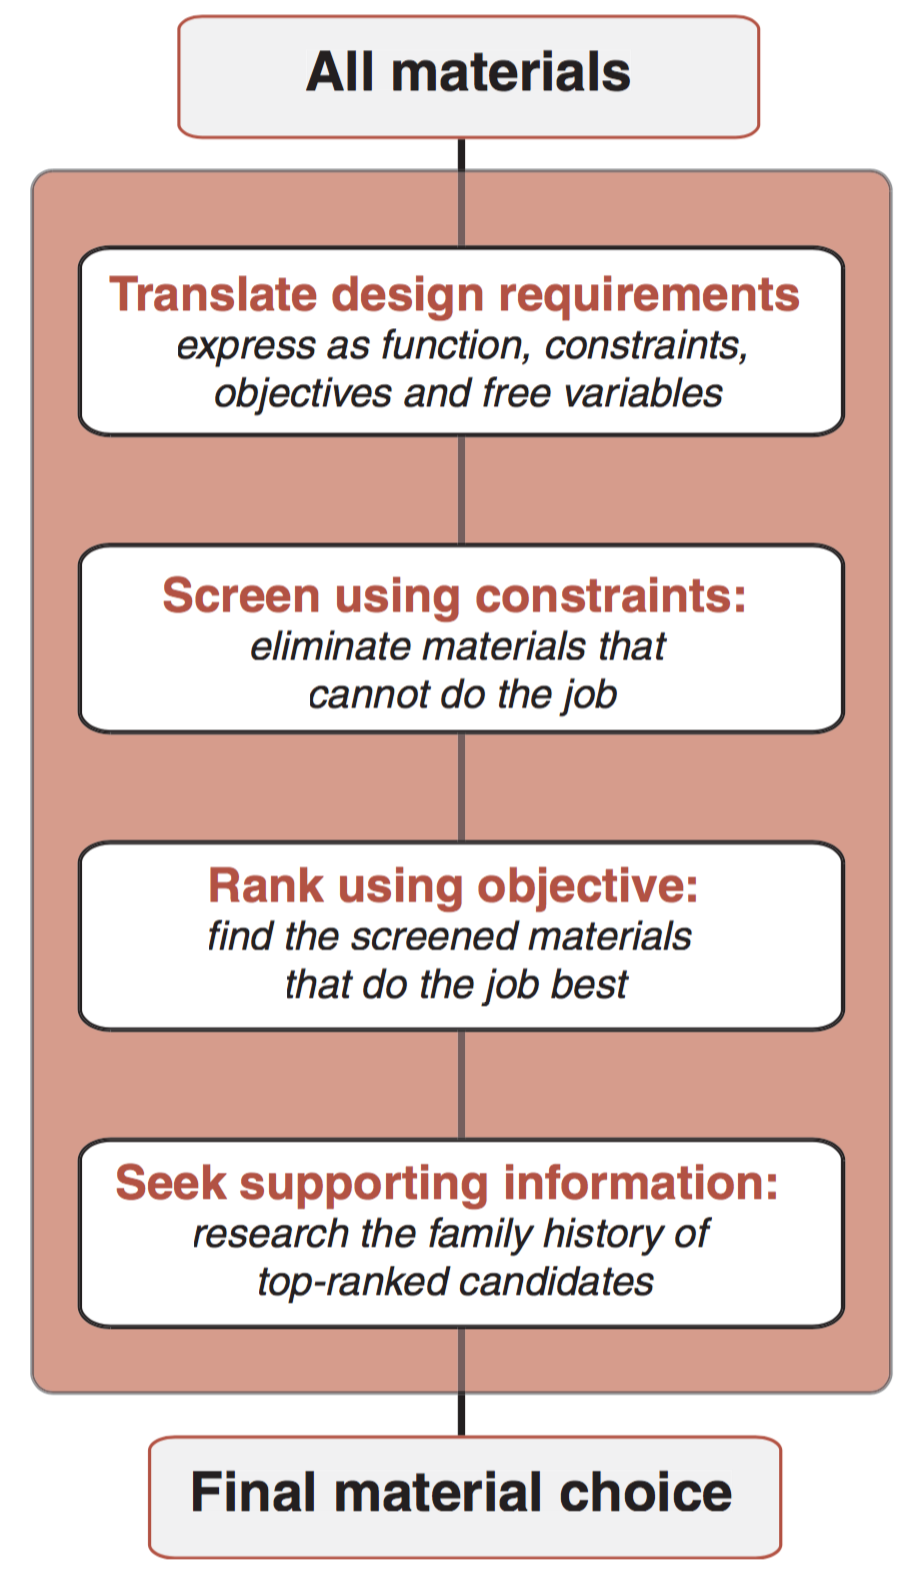
\includegraphics[width=6cm]{Images/MaxImages/AshbyStrat.png}
  \caption{Ashby Materials Selection Strategy, \cite{Ashby05}}
\label{AshbyStrat}
\end{figure}

\subsubsection{Cyclone Materials Selection using Properties Charts}
The materials selection for components of Cyclone was primarily based on the Ashby material property charts. These charts plot material properties against each other to give ratios that are invaluable for selecting a material; examples are strength-density and Young’s modulus-density. 

The desired properties for each component were considered and then the applicable Ashby chart used to determine the most appropriate materials. The most commonly used chart was that of strength against density, as high strength and low weight are required for the majority of components. The chart of Young’s modulus against density was used in tandem with strength-density as the most of the robot’s components must be stiff to withstand the stress it is subjected to during operation. 

\begin{figure}[h!]
\centering
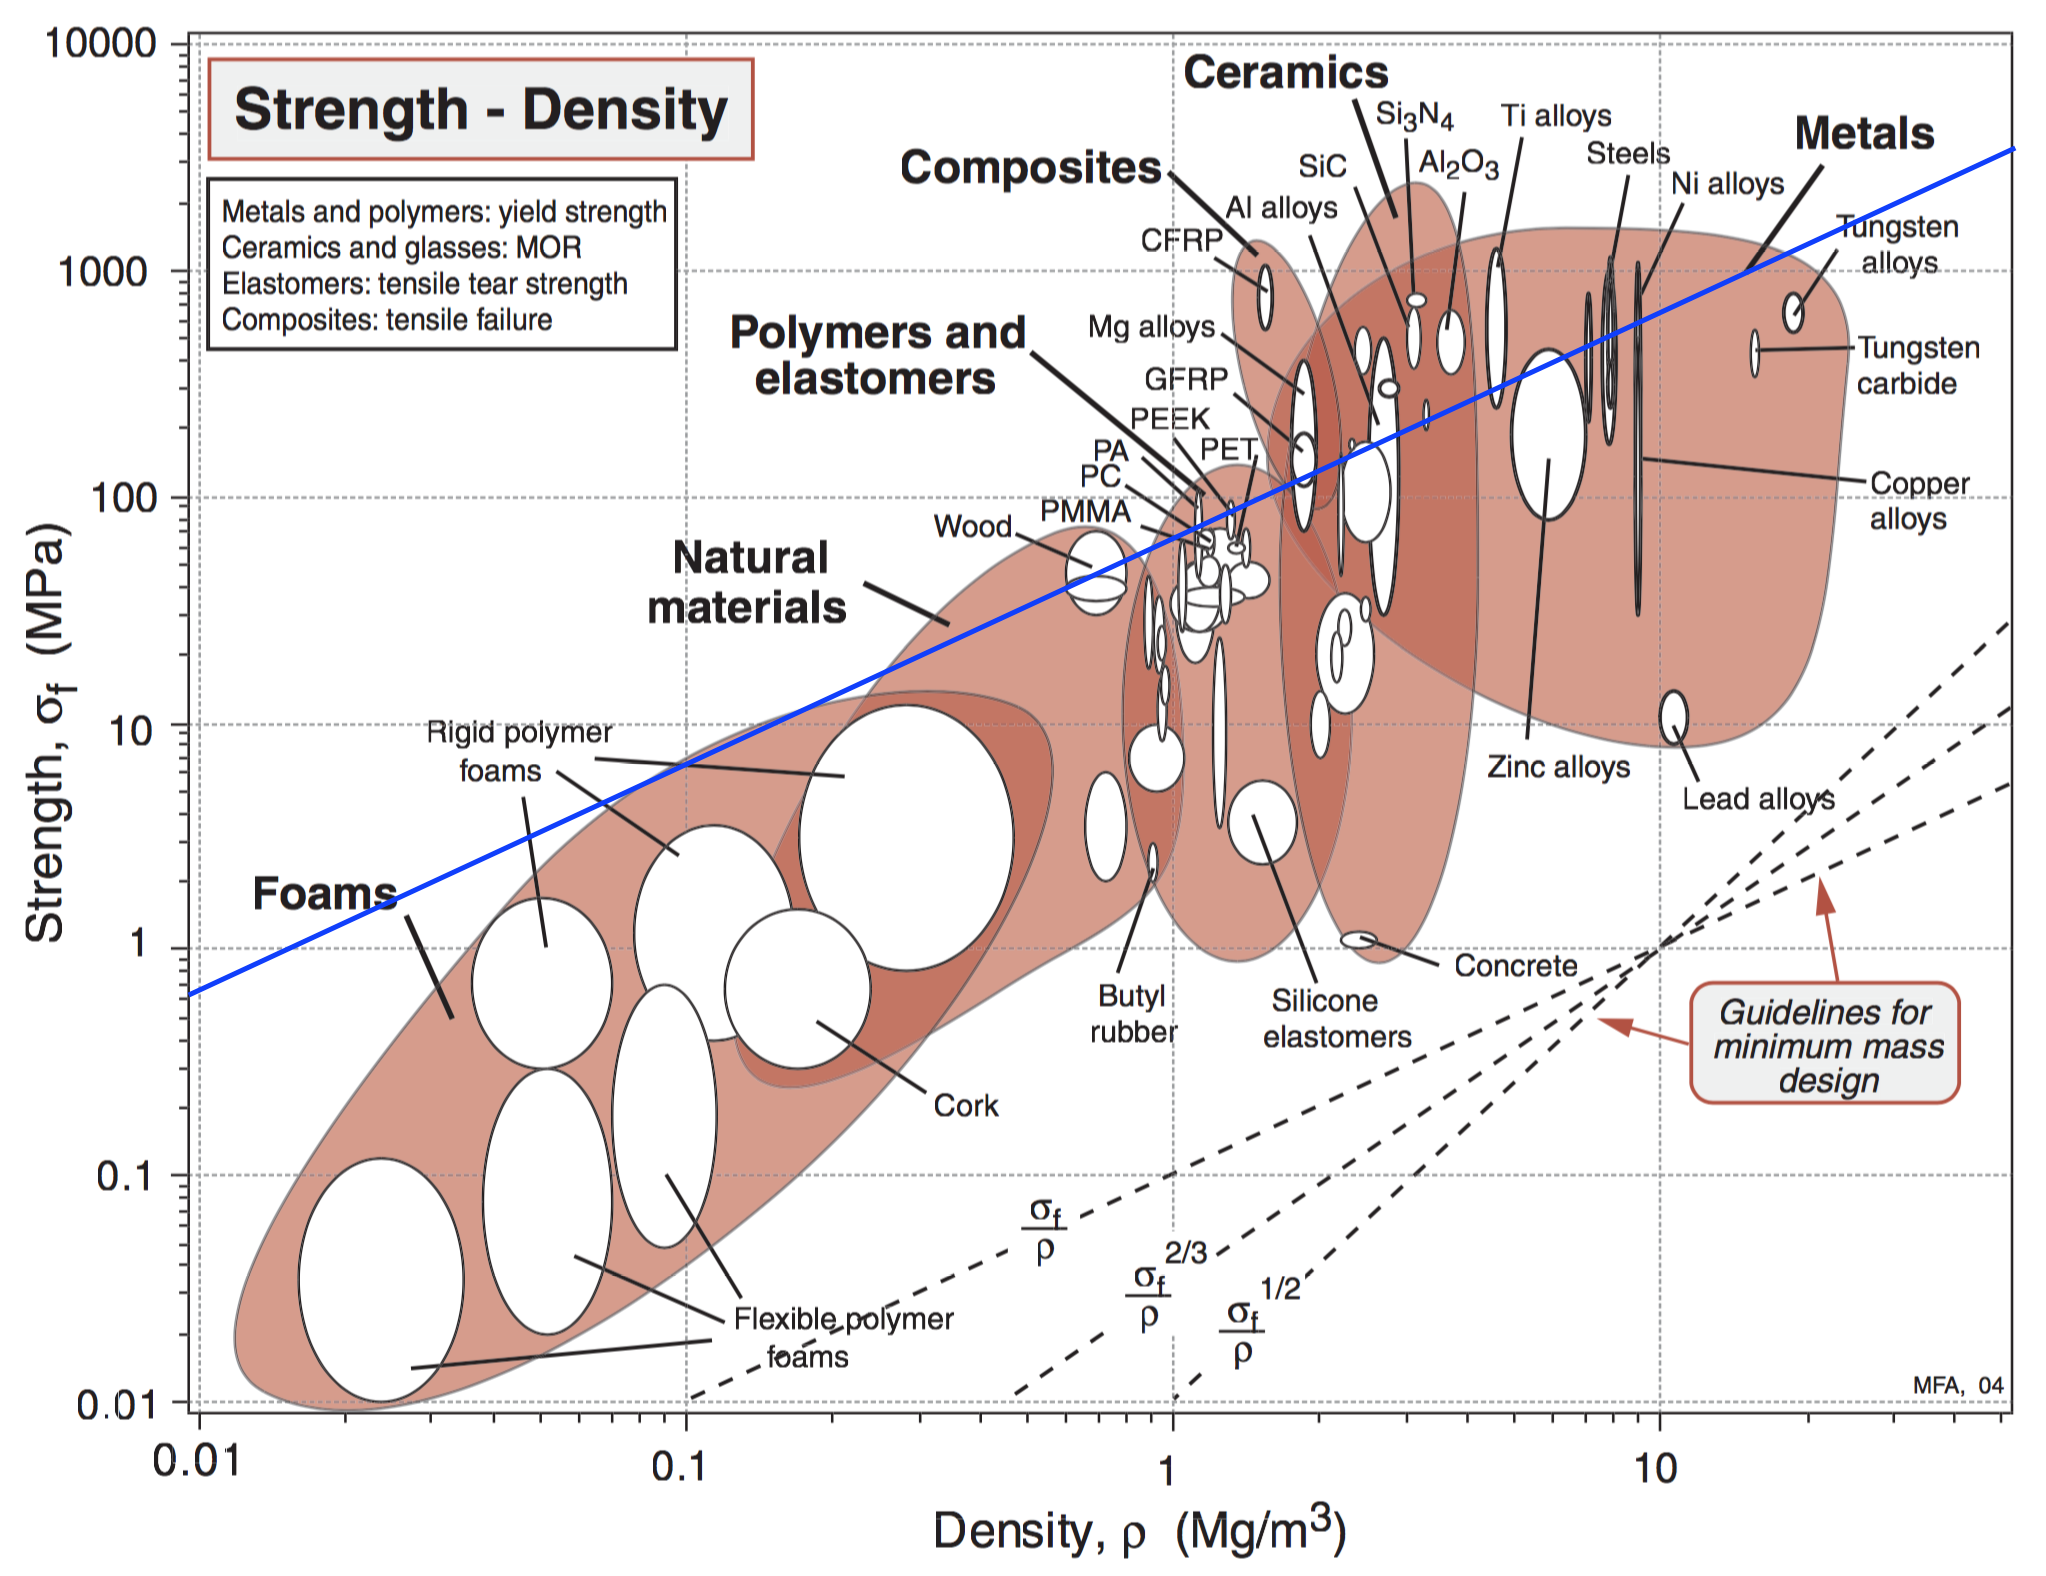
\includegraphics[width=15cm]{Images/MaxImages/StrengthDensity.png}
\caption{Ashby Strength-Density Chart, \cite{Ashby05}}
\label{StrengthDensity}
\end{figure}

\begin{figure}[h!]
\centering
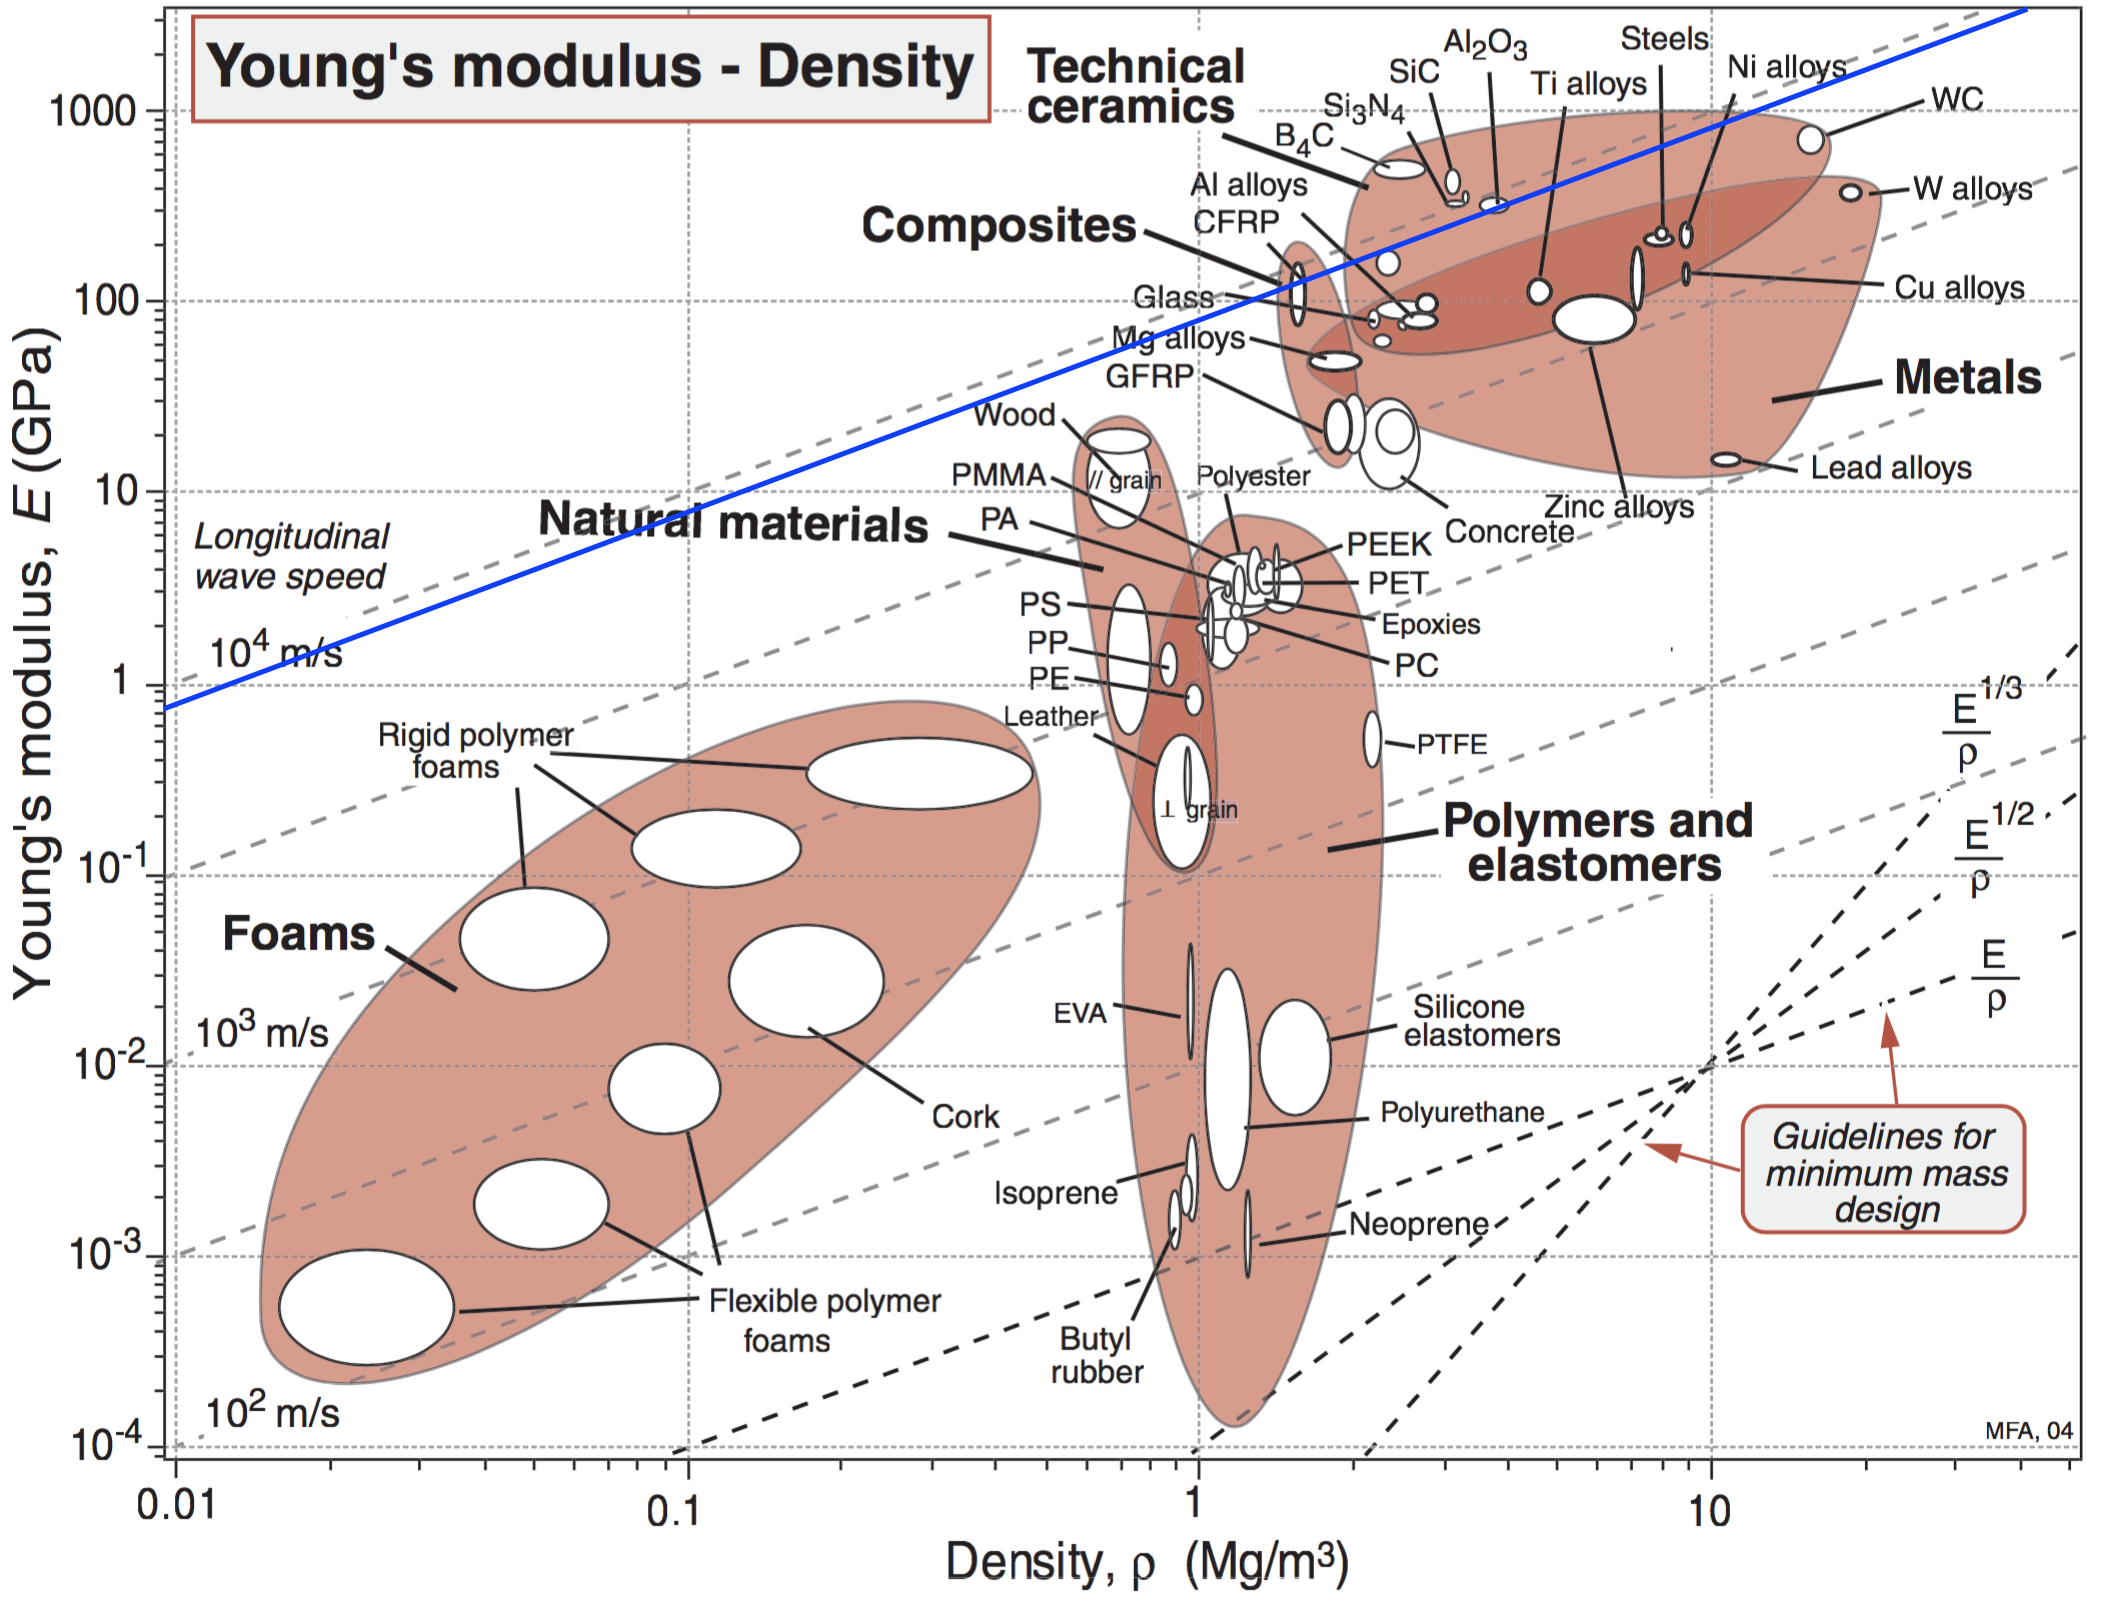
\includegraphics[width=15cm]{Images/MaxImages/YmodDensity.png}
\caption{Ashby Strength-Density Chart, \cite{Ashby05}}
\label{YmodDensity}
\end{figure}

Figures \ref{StrengthDensity} and \ref{YmodDensity} show how the Ashby charts were used to select a suitable material for the chassis. The criteria were high strength, stiffness and low weight, therefore high strength-to-weight and stiffness-to-weight was sought after. The basis material was taken to be aluminium, as it was used in for Orion’s base-plate and Makerbeam is also aluminium. The design guideline for minimum weight was moved upwards to coincide with aluminium and the other materials the line intersected evaluated for viability. Other possible materials were titanium, steels, carbon fibre reinforced plastic, nickel alloys and more. These were then ranked on further criteria. This ranking was carried out using the criteria in Table \ref{CriteriaTable}. N.B. Each attribute is ranked 1-3, the lower number represents a better material attribute. The scores for each criteria were summed and the material with the lowest overall score chosen, as it best fulfils the performance criteria of the design.

\begin{table}[]
\centering
\caption{Material Performance Criteria}
\label{CriteriaTable}
\begin{tabular}{|l|l|l|l|l|l|l|}
\hline
\textbf{Material} & \textbf{Cost} & \textbf{Availability} & \textbf{Manufacture} & \textbf{Corrosion Resistance} & \textbf{Suitability} & \textbf{Total} \\ \hline
\textbf{Al Alloy} &2&1&1&1&1&6\\ \hline
\textbf{Steel} &1&1&1&3&1&7\\ \hline
\textbf{Ni Alloy} &3&3&2&2&1&11\\ \hline
\textbf{Ti Alloy} &3&2&2&1&1&9\\ \hline
\textbf{Mg Alloy} &2&2&2&1&2&9\\ \hline
\textbf{CFRP} &3&2&3&1&3&12\\ \hline
\end{tabular}
\end{table}
\par
Material selection for some parts was carried out using different methods. For example, material selection for the torsion blades was done using the formula to calculate the length of a torsion bar for a given material's Young’s modulus. The material which had needed a length that would give a good range of adjustability was chosen, which was steel. Stainless steel was ultimately chosen for the material’s corrosion resistance, which is needed as the torsion blades are exposed to the environment on the underside of the robot.

This process was carried to determine the most appropriate material for each component. This method of materials selection is beneficial because it incorporates a scientific approach to materials selection, which is often carried out using a “gut feel” approach. Using the Ashby charts means that the most important performance criteria are considered first and all materials compared against where to give a broad range of possible materials which can then be narrowed down.
\subsection{Design For Assembly}
\begin{table}[h]
\centering
\resizebox{\linewidth}{!}{
\begin{tabular}{l c c c c c c c }
\toprule
 &  & \multicolumn{2}{c}{\textbf{Manual Handling}} & \multicolumn{2}{c}{\textbf{Insertion}} & \multicolumn{2}{c}{\textbf{Operation Time}} \\
 \cmidrule(lr){3-4} \cmidrule(lr){5-6} \cmidrule(lr){7-8}
\textbf{Item} & \textbf{QTY} & \textbf{Code} & \textbf{Time (s)} & \textbf{Code} & \textbf{Time (s)} & \textbf{Single (s)} & \textbf{Total (s)} \\
%\multicolumn{1}{l}{Item} & \multicolumn{1}{c}{QTY} & \multicolumn{1}{c}{code} & \multicolumn{1}{c}{Time} \multicolumn{1}{c}{banter} & \multicolumn{1}{c}{Time} & \multicolumn{1}{c}{Single} & \multicolumn{1}{c}{Total}\\
\midrule
\textbf{Attach sideplate to bulkhead} & 2 & & & & & & \\
Place bulkhead upright on table & 1 & 1.0 & 1.5 & \textemdash & \textemdash & 1.5 & 1.5 \\
Place side plate next to bulkhead & 1 & 1.0 & 1.5 & 0.0 & 1.5 & 3 & 3  \\
Screw into place & 3 & 0.1 & 1.43 & 3.9 & 8 & 9.43 & 28.29 \\
\midrule
\textbf{Attach top shell} & 1 & & & & & & \\
Place top shell on assy & 1 & 1.0 & 1.5 & \textemdash & \textemdash & 1.5 & 1.5 \\
Screw into place & 4 & 0.1 & 1.43 & 3.9 & 8 & 9.43 & 37.72 \\
\midrule
\textbf{Attach upper front shell} & 1 & & & & & & \\
Place assy bulkhead-down & 1 & 1.0 & 1.5 & \textemdash & \textemdash & 1.5 & 1.5 \\
Place upper front shell on assy & 1 & 1.0 & 1.5 & 0.0 & 1.5 & 3 & 3 \\
Screw into place & 4 & 0.1 & 1.43 & 3.9 & 8 & 9.43 & 37.72 \\
\midrule
\textbf{Attach lower front shell} & 1 & & & & & & \\
Place lower front shell on assy & 1 & 1.0 & 1.5 & \textemdash & \textemdash & 1.5 & 1.5 \\
Screw into place & 4 & 0.1 & 1.43 & 3.9 & 8 & 9.43 & 37.72 \\
\midrule
\textbf{Attach upper front shell} & 1 & & & & & & \\
Place assy bulkhead-down & 1 & 1.0 & 1.5 & \textemdash & \textemdash & 1.5 & 1.5 \\
Place upper front shell on assy & 1 & 1.0 & 1.5 & 0.0 & 1.5 & 3 & 3 \\
Screw into place & 4 & 0.1 & 1.43 & 3.9 & 8 & 9.43 & 37.72 \\
\midrule
\multicolumn{3}{l}{\textbf{Front Module Total Assembly Time}} & \multicolumn{5}{c}{\textbf{231.46}}\\
\bottomrule
\end{tabular}
}
\caption{Boothroyd-Dewhurst analysis of Cyclone's Front Module}
\label{tab:boothcyclonefm}
\end{table}


%\section{Testing}
%\subsection{Electronics Testing}
\subsubsection{Control Results}
Control of Cyclones motors via a PS3 controller over a network was tested. [FIGURE BELOW] shows the ROS node connections, it is generated from the in built ‘rqt\_graph' function. This proves the connections with topic successful published and subscribed to by each node.\par

%[FIGURE – RQT_GRAPH LABELLED]

This was achieved with the 2 launch files as discussed previously. Each of these files were launched from the laptop, by connecting to the robot’s Pico board via a secure shell (SSH).\par

%[FIGURE – LAUNCH FILES LABELLED]

\subsubsection{Control Critical Analysis}
In order to achieve the best results with Cyclone, continuous testing was performed over the entirety of the project. One issue that was overcome, was the inherent PWM jitter due to the use of a low-cost Arduino micro-controller. This caused the motors to judder at zero velocity, as the duty ratio was not exactly 50:50. So not only would the robot move when it was expected to be stationary, but this also induced a large current draw due to the rapid changes in inertia. This was overcome by the introduction of an enable signal. This signal would fall low at a command for 0 velocity, shutting down the motors to ensure they were stationary.\par

Secondly, there was an issue with ground loops and the correct galvanic isolation. These ground loops caused a difference in potential in the ground lines so the PWM signal output was floating. In addition, by reconfiguring the grounding scheme it prevented a large conducting current path through the communications ground line. An issue faced by last years team was inadequate grounding of the controllers units, which caused the USB controller IC in within the device to blow.\par

\subsubsection{Battery Monitoring Results}
The battery monitor board was tested and proved to produce the expected regulated outputs of 5V and 12V. The on-board ATmega328 functioned as expected;, being capable of shutting down the motors, monitoring the cell voltages and updating the LED board.\par

\subsubsection{Battery Monitoring Critical Analysis}
Although the board output a stable 12V, this dropped once loaded by the Pico board, and could not match the power demand placed upon it. This was overcome by changing R14 from 10kΩ to 330Ω, so the zener diodes reverse breakdown voltage in the latching circuitry was still reached with the increased load. Furthermore, the LED was removed as it was holding the micro-controller in reset by not allowing the current to flow into the ATmega328 pin. Equally, this could have been overcome by decreasing the value of the pullup resistor, if the operation of the LED was required.\par

Besides the modifications stated above, only aesthetics would need to be modifying on a 2nd revision of the board. This would include, increasing the distance between the connectors to allow the wires greater freedom of movement and to allow the underlying silkscreens to be seen. Furthermore, making the pads larger would make solderijng easier.\par

Finally, the regulators were intended to reside on the reverse side of the board to aid with heat dissipation to the chassis. However, due to a misunderstanding in the software they were mounted on the topside. It does not alter the performance of the board, but would be desirable to have them as they were intended.\par

%[FIGURE – ACTUAL SOLDERED BAORD WITH USB ADAPTOR BOARD]

\subsubsection{Robot Battery Life}
This design of Cyclone considers the use of one Thunder Power 5000mAh LiPo battery. Therefore, in the worse case scenario of the motors running at full power (i.e: continuously up a standard stair angle) with the power draws as given in table \ref{tab:pwrreq}, the robot would last for $\approx$20 minutes. However, this is unlikely to be the case with a better approximation being $\approx$30 minutes, when under more ‘normal’ operating conditions. These approximations are inherently difficult to calculate due to the real-world effects associated with current draws and battery discharge rates. In the future, if required, a second battery could be incorporated to power an arm, or to increase the robot’s battery life should it be required for the competition.\par


%\section{Future Recommendations}

% WRITE AS A GROUP %

% SOME ELECTRONICS SUGGESTIONS - EXPAND ON THIS POINTS, THEY ARE JUST FOR IDEAS!
% - Incorporate remaining sensors
% - Opto-couplers for heartbeats to avoid ground loops like mentioned in the testing results.
% - Re-writing code to increase system’s responsiveness if required.
% - Battery monitor software currently set up for 2 heartbeats only?

\clearpage
\section{References}
%% References
%%
%% Following citation commands can be used in the body text:
%% Usage of \cite is as follows:
%%   \cite{key}          ==>>  [#]
%%   \cite[chap. 2]{key} ==>>  [#, chap. 2]
%%   \citet{key}         ==>>  Author [#]

%% References with bibTeX database:

\bibliographystyle{model1-num-names}
\bibliography{sample.bib}





\end{document}

%%
%% End of file `elsarticle-template-1-num.tex'.